\documentclass{article}

\usepackage{amsmath, amsthm, amssymb, amsfonts}
\usepackage{thmtools}
\usepackage{graphicx}
\usepackage{setspace}
\usepackage{geometry}
\usepackage{float}
\usepackage{hyperref}
\usepackage[utf8]{inputenc}
\usepackage[english]{babel}
\usepackage{framed}
\usepackage[dvipsnames]{xcolor}
\usepackage{tcolorbox}

%Define the listing package
\usepackage{listings} %code highlighter
\usepackage{color} %use color
\definecolor{mygreen}{rgb}{0,0.6,0}
\definecolor{mygray}{rgb}{0.5,0.5,0.5}
\definecolor{mymauve}{rgb}{0.58,0,0.82}
 
%Customize a bit the look
\lstset{ %
backgroundcolor=\color{white}, % choose the background color; you must add \usepackage{color} or \usepackage{xcolor}
basicstyle=\footnotesize, % the size of the fonts that are used for the code
breakatwhitespace=false, % sets if automatic breaks should only happen at whitespace
breaklines=true, % sets automatic line breaking
captionpos=b, % sets the caption-position to bottom
commentstyle=\color{mygreen}, % comment style
deletekeywords={...}, % if you want to delete keywords from the given language
escapeinside={\%*}{*)}, % if you want to add LaTeX within your code
extendedchars=true, % lets you use non-ASCII characters; for 8-bits encodings only, does not work with UTF-8
frame=single, % adds a frame around the code
keepspaces=true, % keeps spaces in text, useful for keeping indentation of code (possibly needs columns=flexible)
keywordstyle=\color{blue}, % keyword style
% language=Octave, % the language of the code
morekeywords={*,...}, % if you want to add more keywords to the set
numbers=left, % where to put the line-numbers; possible values are (none, left, right)
numbersep=5pt, % how far the line-numbers are from the code
numberstyle=\tiny\color{mygray}, % the style that is used for the line-numbers
rulecolor=\color{black}, % if not set, the frame-color may be changed on line-breaks within not-black text (e.g. comments (green here))
showspaces=false, % show spaces everywhere adding particular underscores; it overrides 'showstringspaces'
showstringspaces=false, % underline spaces within strings only
showtabs=false, % show tabs within strings adding particular underscores
stepnumber=1, % the step between two line-numbers. If it's 1, each line will be numbered
stringstyle=\color{mymauve}, % string literal style
tabsize=2, % sets default tabsize to 2 spaces
title=\lstname % show the filename of files included with \lstinputlisting; also try caption instead of title
}
%END of listing package%
 
\definecolor{darkgray}{rgb}{.4,.4,.4}
\definecolor{purple}{rgb}{0.65, 0.12, 0.82}
 
%define Javascript language
\lstdefinelanguage{JavaScript}{
keywords={typeof, new, true, false, catch, function, return, null, catch, switch, var, if, in, while, do, else, case, break, @},
keywordstyle=\color{blue}\bfseries,
ndkeywords={class, export, boolean, throw, implements, import, this},
ndkeywordstyle=\color{darkgray}\bfseries,
identifierstyle=\color{black},
sensitive=false,
comment=[l]{//},
morecomment=[s]{/*}{*/},
commentstyle=\color{purple}\ttfamily,
stringstyle=\color{red}\ttfamily,
morestring=[b]',
morestring=[b]"
}
 
\lstset{
language=JavaScript,
extendedchars=true,
basicstyle=\footnotesize\ttfamily,
showstringspaces=false,
showspaces=false,
numbers=left,
numberstyle=\footnotesize,
numbersep=9pt,
tabsize=2,
breaklines=true,
showtabs=false,
captionpos=b
}

\colorlet{LightGray}{White!90!Periwinkle}
\colorlet{LightOrange}{Orange!15}
\colorlet{LightGreen}{Green!15}

\newcommand{\HRule}[1]{\rule{\linewidth}{#1}}

\NewEnviron{NORMAL}{% 
    \scalebox{2}{$\BODY$} 
} 

\declaretheoremstyle[name=Theorem,]{thmsty}
\declaretheorem[style=thmsty,numberwithin=section]{theorem}
\tcolorboxenvironment{theorem}{colback=LightGray}

\declaretheoremstyle[name=Proposition,]{prosty}
\declaretheorem[style=prosty,numberlike=theorem]{proposition}
\tcolorboxenvironment{proposition}{colback=LightOrange}

\declaretheoremstyle[name=Principle,]{prcpsty}
\declaretheorem[style=prcpsty,numberlike=theorem]{principle}
\tcolorboxenvironment{principle}{colback=LightGreen}

\setstretch{1.2}
\geometry{
    textheight=9in,
    textwidth=5.5in,
    top=1in,
    headheight=12pt,
    headsep=25pt,
    footskip=30pt
}

% ------------------------------------------------------------------------------

\begin{document}

% ------------------------------------------------------------------------------
% Cover Page and ToC
% ------------------------------------------------------------------------------

\title{ \normalsize \textsc{}
		\\ [2.0cm]
		\HRule{1.5pt} \\
		\LARGE \textbf{\uppercase{Architetture degli Elaboratori}
        Architetture e Sistemi Operativi - I Semestre
		\HRule{2.0pt} \\ [0.6cm] \LARGE{Corso A} \vspace*{10\baselineskip}}
		}
        
\date{\text{Ultima Compilazione - }\today}

\author{\textbf{Autore} \\ 
		Giuseppe Acocella \\
		2024/25\\
        \url{https://github.com/Peenguino}}

\maketitle
\newpage

\tableofcontents

\newpage

\section{Introduzione}

\subsection{Astrazione a livelli}

Un calcolatore elettronico si basa su dei livelli di astrazione:

\begin{figure}[htbp]
    \center
    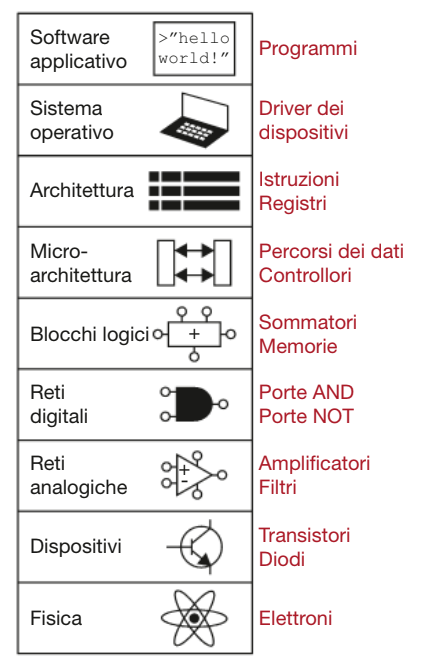
\includegraphics[scale=0.6]{img/livelliAstrazione.png}
    \paragraph{Interfacce}
Questi livelli permettono di creare una gerarchia, stabiliscono una comunicazione tra i livelli stessi grazie a delle \textbf{interfacce}. Un livello $n+1$ infatti si basa su elementi composti del livello $n$. Ad esempio, le porte logiche del livello \textit{circuiti} si basa sulla composizionalità di elementi del livello \textit{device}.
\end{figure}


\begin{figure}[htbp]
    \center
    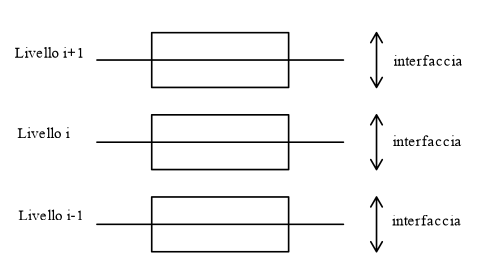
\includegraphics[scale=0.55]{img/interfaccia.png}
\end{figure}

\newpage

\paragraph{Gerarchia, modularità e regolarità}

Definita quindi l'astrazione, che ci permette di ragionare più ad alto livello, allontanandoci dall'implementazione e realizzazione fisica di un calcolatore, dobbiamo introdurre tre regole che vanno rispettate per mantenere una lineare crescita ed evoluzione dei calcolatori:

\begin{enumerate}
    \item \textbf{Gerarchia}: Ogni livello ha uno specifico posto.
    \item \textbf{Regolarità}: Ogni elemento ha una struttura regolare costante che permette una composizione scalabile.
    \item \textbf{Modularità}: Ogni elemento può essere utilizzato in composizioni diverse, mantenendo la sua struttura.
\end{enumerate}

\subsection{Sistema Binario}

Il \textbf{sistema binario} è un sistema \textbf{posizionale}, ha base $2$. che utilizza come cifre \{ 0,1 \}. 

\[ 2^{2} * 1 + 2^{1} * 1 + 2^{0} * 0 = 6_{(10)} \]

\subsubsection{Complemento a Due}

Il complemento a due nel sistema binario permette la rappresentazione dei numeri relativi. Il bit più significativo indica il segno (0 segno positivo, 1 segno negativo). Mostriamo un esempio su 1 byte dedicato alla rappresentazione di un numero in base 10. Anche per poter leggere un numero post complemento a due, e convertirlo in base 10, va ricordato il bit più significativo applicando gli stessi passi. Mostriamo il complemento a due di $3_{10}$.

\begin{figure}[htbp]
    \center
    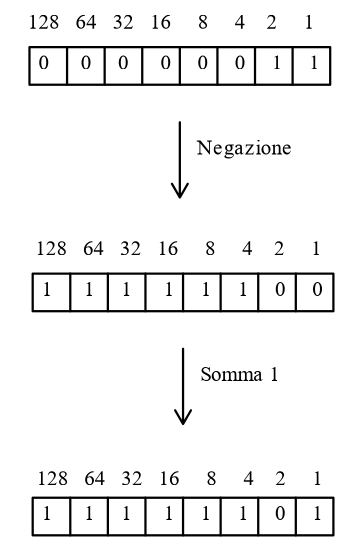
\includegraphics[scale=0.6]{img/complementoDue.png}
\end{figure}

\newpage

\paragraph{Numeri con virgola mobile}

Simile è la rappresentazione dei numeri con la virgola. Il numero stesso sarà infatti rappresentato da una mantissa e da un esponente. Verranno quindi dedicati dei bit alla mantissa, un bit al segno e i restanti all'esponente, in base a quale sia il focus del tipo con virgola mobile in questione.

\subsection{Porte Logiche}

Introduciamo le porte logiche, ossia la rappresentazione in livello componenti degli operatori logici $AND, OR, NOT$:

\begin{enumerate}

    \item \textbf{Porta AND}:
        \begin{figure}[htbp]
            \center
            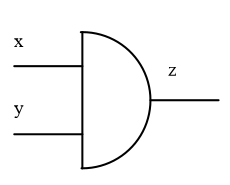
\includegraphics[scale=0.45]{img/portaAND.png}
        \end{figure}

    \item \textbf{Porta OR}:
        \begin{figure}[htbp]
            \center
            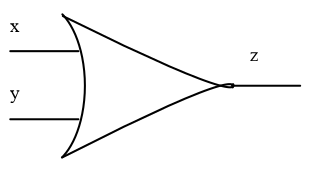
\includegraphics[scale=0.45]{img/portaOR.png}
        \end{figure}

    \item \textbf{Porta NOT}:
        \begin{figure}[htbp]
            \center
            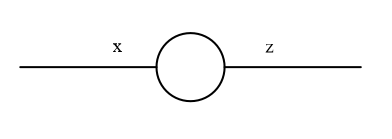
\includegraphics[scale=0.45]{img/portaNOT.png}
        \end{figure}    

\end{enumerate}

Ricordiamo che questo tipo di porte accetta due input $ \{ x,y \} $ e produce un output $z$.

Vedremo più avanti in che occasioni è possibile aumentare il numero di input e l'effetto sul circuito complessivo.

\paragraph{Map dei valori 0-1} E' necessario stabilire una correlazione tra voltaggio e bit rappresentato. Solitamente:

\begin{multline}
    \\ 0 \mapsto 0 \: volt \\
    \\ 1 \mapsto 3/5/12 \: volt \\
\end{multline}

\newpage

\vspace*{25px}

\paragraph{Map operatori} Per poter esprimere più facilmente espressioni articolate, anche gli operatori vengono mappati:

\begin{multline}
    \\ AND(x,y) \: \mapsto \: x \: * \: y \\
    \\ OR(x,y) \: \mapsto \: x \: + \: y \\
    \\ NOT(x) \: \mapsto \: \overline{x} \\
\end{multline}

\vspace*{50px}

\subsubsection{Composizionalità di porte}

Possiamo comporre le porte per rappresentare espressioni logiche più complesse:

\begin{equation}
    NOT \: (x \: AND \: y)
\end{equation}

    \begin{figure}[htbp]
        \center
        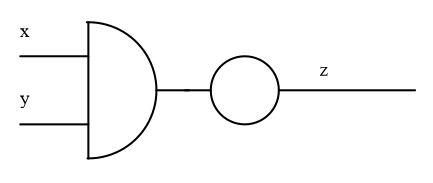
\includegraphics[scale=0.45]{img/exp1.png}
    \end{figure}

\begin{equation}
    NOT (x) \: OR \: y
\end{equation}

    \begin{figure}[htbp]
        \center
        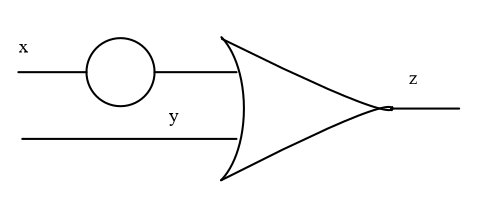
\includegraphics[scale=0.45]{img/exp2.png}
    \end{figure}    

\newpage

\section{Logica Combinatoria e Sintesi Standard}

Come realizziamo un circuito basandoci sulla descrizione ad alto livello di un problema?
Bisogna seguire un preciso algoritmo che sviluppi una tabella di verità rispetto alle variabili in questione e che interpreti i dati prodotti.

\subsection{Parità di Stringa di Bit} Mostriamo l'algoritmo in questione su questo esempio:

\begin{enumerate}
    \item \textbf{Descrizione funzione}: Se numero di bit settati a $1$ è pari allora torna 1, altrimenti 0.
    \item \textbf{Tabella di verità}: Sviluppo la tabella e noto quali valori mi permettono di produrre $1$ in output.

    \begin{figure}[htbp]
        \center
        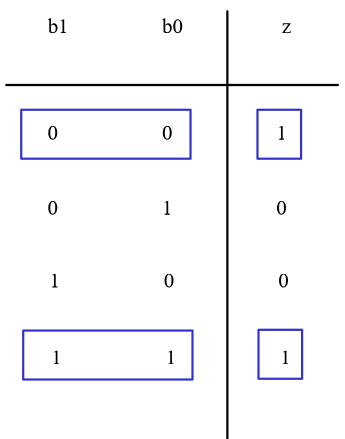
\includegraphics[scale=0.5]{img/tabellaVeritaBitParita.png}
    \end{figure}

    \item \textbf{Espressione associata}: Seleziono le variabili delle stesse righe dei vari $1$ in output e
    \begin{enumerate}
        \item Nego la variabile se è settata a $0$.
        \item Non la nego se la variabile è settata a $1$.
    \end{enumerate}

    \begin{equation}
        z \: = \: \overline{b_{1}} \: \overline{b_{0}} \: + \: b_{1}\:b_{0} 
    \end{equation}

    \item \textbf{Rappresentazione Circuito}: Possiamo dunque rappresentare l'espressione in questione in formato circuito:

    \begin{figure}[htbp]
        \center
        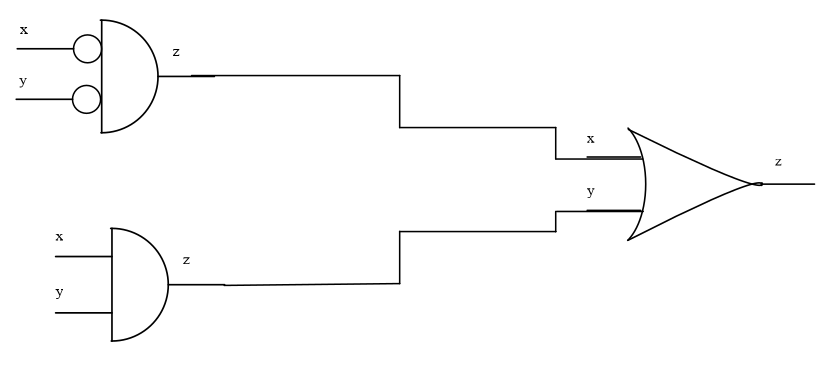
\includegraphics[scale=0.42]{img/expCircuito1.png}
    \end{figure}
    
\end{enumerate}

\newpage

\subsection{Numero Porte e Costo in Tempo}

A livello elettrico, per poter raggiungere il voltaggio richiesto durante il map dei bit, sarà necessario attendere del tempo:

    \begin{figure}[htbp]
        \center
        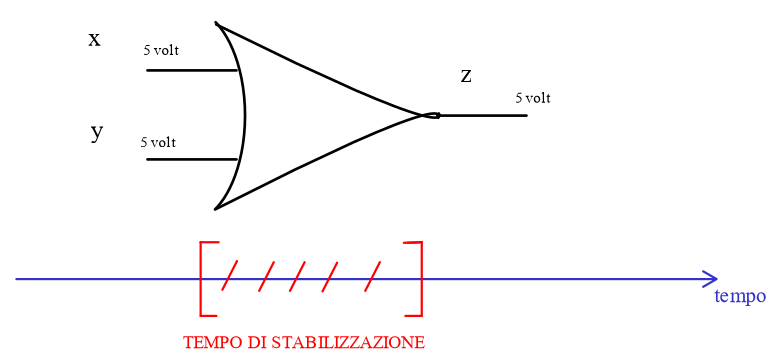
\includegraphics[scale=0.55]{img/deltaTempo.png}
    \end{figure}

Questo viene chiamato \textbf{tempo di stabilizzazione}. Questo dipende anche dal numero di ingressi delle porte in questione. Oltre gli $8$ ingressi è dimostrata l'inefficienza del circuito composto da porte di questo tipo. Solitamente indichiamo il costo dell'attraversamento di una colonna di porte con $\Delta t$.

\vspace*{15px}

\subsection{Multiplexer e Composizionalità}

Mostriamo un multiplexer (\textbf{livello circuiti}) formato dalla composizione di varie porte logiche (\textbf{livello componenti}) secondo le regole della \textbf{logica combinatoria}.

\begin{enumerate}

    \item \textbf{Descrizione Funzione e Tabella}: Descriviamo la funzione che vogliamo rappresentare in circuito e successivamente produciamo la relativa tabella di verità.

    \begin{enumerate}
        \item Se $c = 1 \Rightarrow z \mapsto a$
        \item Se $c = 0 \Rightarrow z \mapsto b$
    \end{enumerate}

    \begin{figure}[htbp]
        \center
        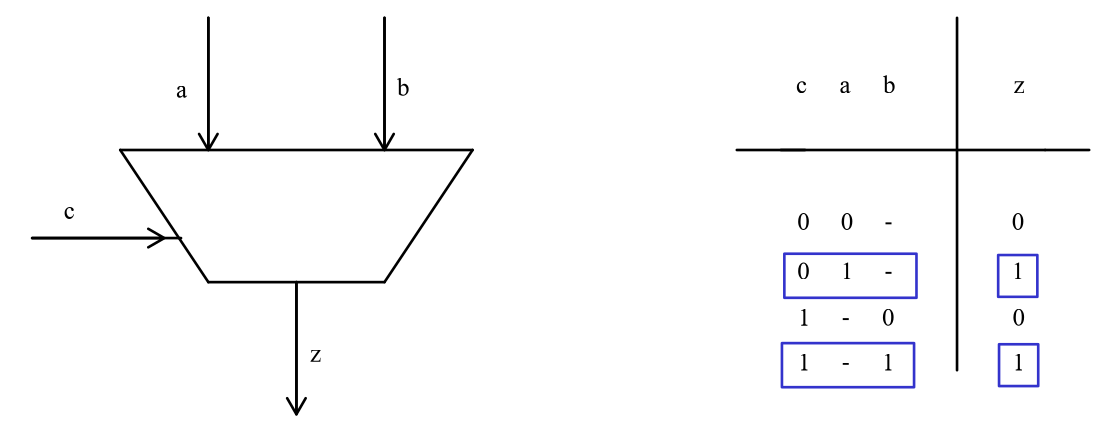
\includegraphics[scale=0.45]{img/multiplexer.png}
        %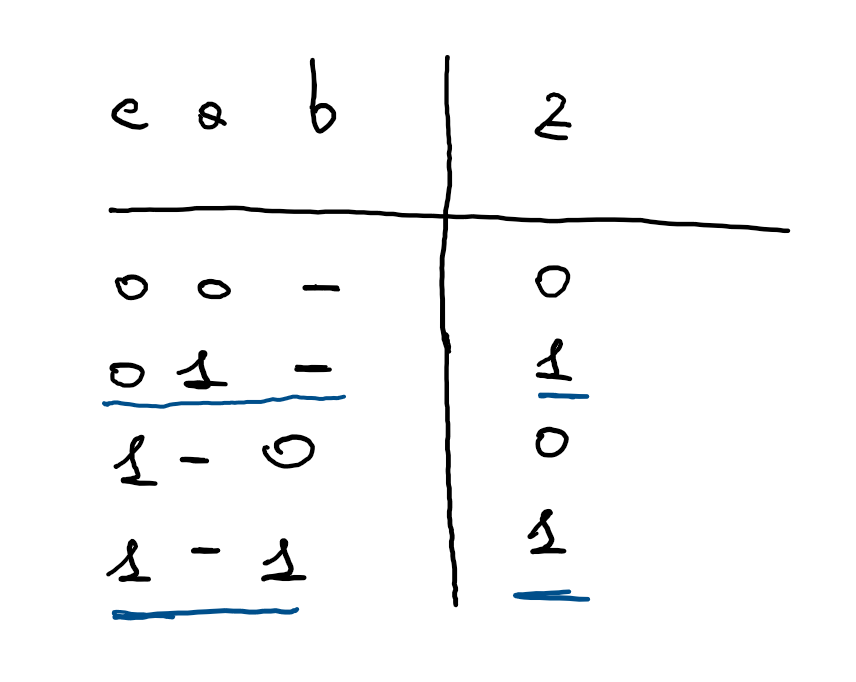
\includegraphics[scale=0.23]{img/tabellaVerita2.png}
    \end{figure}

    \newpage
    
    \item \textbf{Espressione associata}: Descriviamo dunque l'espressione osservando la tabella di verità. Notiamo che nella prima riga e nella quarta, rispettivamente $b$ e $a$ possono assumere qualsiasi valore.

    \begin{multline}
        \\ z \: = \: \overline{c}\:a\:(b \: + \: \overline{b}) \: + \: c\:(a \: + \: \overline{a}) \: = \\
        \\ = \: \overline{c}\:a \: + \: c \: b \\
    \end{multline}

    \item \textbf{Rappresentazione Circuito}: Osserviamo il circuito corrispondente.

    \begin{figure}[htbp]
        \center
        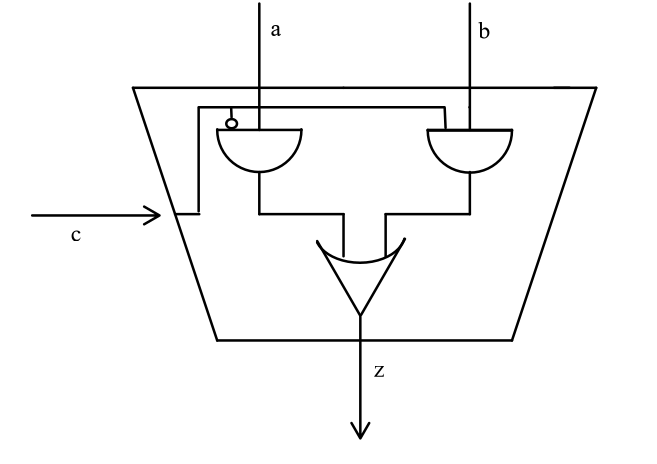
\includegraphics[scale=0.3]{img/multiplexer1.png}
    \end{figure}

    Sarà possibile d'ora in poi utilizzare il \textbf{multiplexer} come unità del livello di astrazione \textbf{circuiti}. Abbiamo però avuto la dimostrazione di come si compone di unità del livello sottostante \textbf{componenti}.
    
\end{enumerate}    

\vspace*{20px}

\subsection{Composizione/Elementi Ex-Novo}

Dato che abbiamo introdotto il tempo di stabilizzazione $\Delta t$ possiamo valutare quale approccio sia più efficiente tra:
\begin{enumerate}
    \item Composizione di oggetti già esistenti del livello sottostante nella gerarchia dei livelli di astrazione.
    \item Progettazione di nuove componenti, aumentando il livello di porte e costruendolo su misura alla formula corrente.
\end{enumerate}

Mostriamo un esempio nella pagina successiva.

\newpage

\paragraph{Multiplexer a 2 entrate a 2 bit} Definiamo prima la sua formula e la corrispondente tabella di verità. Successivamente lo rappresenteremo con due reti diverse.

\begin{enumerate}
    \item \textbf{Descrizione Funzione e Tabella}: Assumiamo di avere due entrate da due bit $a,b$, un entrata di controllo $c$ ed un uscita da due bit. Vogliamo quindi che se $c = 0$, allora in output avremo il valore di $a$, mentre quello di $b$ se $ c = 1 $.
    \begin{figure}[htbp]
        \center
        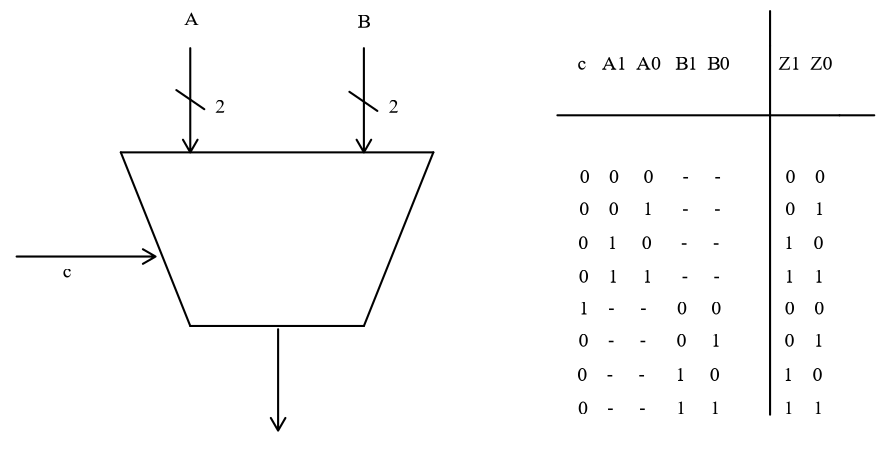
\includegraphics[scale=0.4]{img/multiplexerInput2.png}
        %\includegraphics[scale=0.3]{img/tabellaVeritàMltplxr2.png}
    \end{figure}

    \item \textbf{Espressione Associata}: Osservando la tabella, produciamo l'espressione, composta dalla rappresentazione di $b1,b2$

    \begin{enumerate}
        \item $z_{1} = \overline{C}A_{1}\overline{A_{0}} + \overline{C}A_{1}A_{0} + CB_{1}\overline{B_{0}} + CB_{1}B_{0}$
        \item $z_{0} = \overline{C}\overline{A_{1}}A_{0} + \overline{C}A_{1}A_{0} + C\overline{B_{1}}B_{0} + CB_{1}B_{0}$
    \end{enumerate}

    \item \textbf{Reti}: Possiamo rappresentarne diversi tipi.
    \begin{enumerate}
        \item \textbf{Rappresentazione Nuova}: Si basa su porte $AND$ da tre ingressi (prima colonna) e porte $OR$ da quattro ingressi (seconda colonna). Tempo di stabilizzazione $2\Delta t$.
        \begin{figure}[htbp]
        \center
        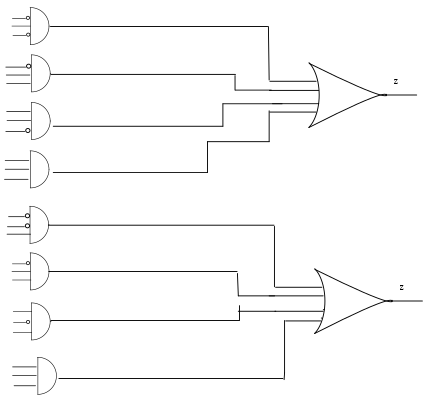
\includegraphics[scale=0.475]{img/implementazione1Mltplxr.png}
    \end{figure}
    \item \textbf{Rappresentazione Composta}: Potremmo anche utilizzare 2 multiplexer in prima colonna e uno nella seconda per poter ricavare lo stesso risultato. Questo è un raro caso in cui le due implementazioni causano lo stesso costo. Solitamente un implementazione nuova permette un ottimizzazione del costo di stabilizzazione provocato.
    \end{enumerate}
    
\end{enumerate}

\newpage

\subsection{Valutazione del costo di stabilizzazione approssimata}

A volte è necessario valutare quanto ci costa implementare ex novo un espressione logica. Dunque eseguiamo questi passaggi:

\begin{enumerate}
    \item \textbf{Numero righe e termini in AND}
    
    Visualizziamo la tabella logica, notiamo quanti $k$ input abbiamo. Possiamo dunque stabilire che la tabella produrrà $2^{k}-1$ termini in and composti tra gli input. Dunque possiamo stabilire questa come prima "colonna" del costo complessivo di stabilizzazione.

    \item \textbf{Altezza dell'albero}

    Ricordando che il massimo di entrate ottimali in una porta è pari ad $8$ allora possiamo determinare l'attuale numero di input $k$ come base di un logaritmo, dove l'argomento sarà appunto $2^{k}-1$.

    \[ ceil \: [ \: log_{k} ( \:2^{k}-1 \: )\:]  \]
\end{enumerate}

Sommando quindi questi due livelli, otteniamo un approssimazione del costo di stabilizzazione totale della tabella di verità implementata ex novo.

\subsection{Full Adder}

Il Full Adder permette di eseguire somme con riporto in colonna. Questo avrà quindi:
\begin{enumerate}
    \item \textbf{Input}: Due bit in input che vogliamo sommare.
    \item \textbf{Riporto in ingresso}: Di default settato a $0$.
    \item \textbf{Riporto in uscita}: Se la somma dei due bit "sfora" viene prodotto in output un riporto.
    \item \textbf{Output}: Somma dei due bit in ingresso.
\end{enumerate}

\begin{figure}[htbp]
        \center
        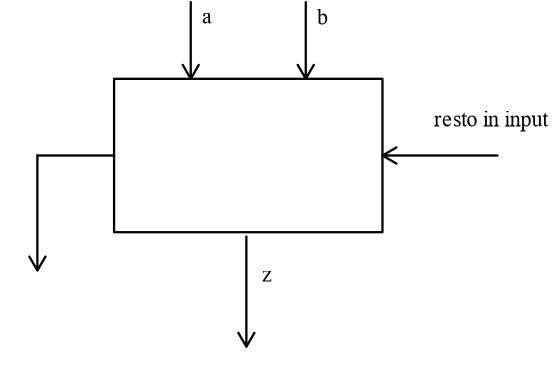
\includegraphics[scale=0.55]{img/fullAdder.png}
    \end{figure}

\newpage

\subsubsection{Valutazione costo Full Adder 8 bit in ingresso}

Valutiamo il costo delle implementazioni di un full adder con 8 bit in ingresso.

\vspace*{25px}

\begin{enumerate}
    \item \textbf{Composizione di Full Adder}: Assumiamo che un Full Adder singolo costi $2\Delta t$. Dobbiamo dunque impostare questa rete:
    \begin{figure}[htbp]
        \center
        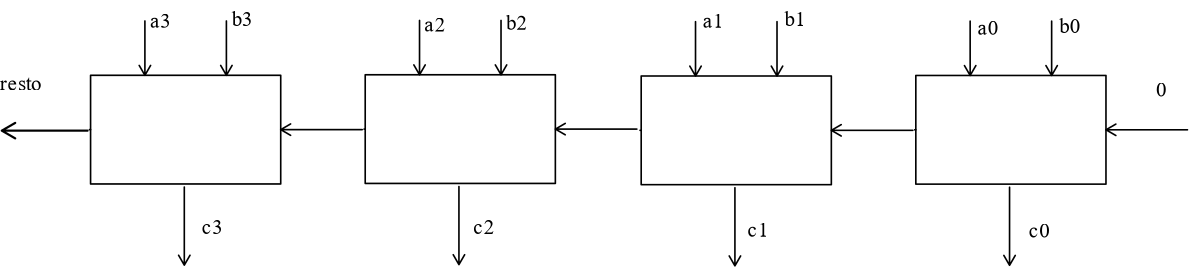
\includegraphics[scale=0.4]{img/fullAdder8bit1.png}
        
        Questa implementazione costa quindi $8\Delta t$.
    \end{figure}

    \vspace*{25px}
    
    \item \textbf{Implementazione Ex Novo}: Abbiamo stabilito di avere $8$ bit in ingresso. 
    \begin{enumerate}
        \item \textbf{Colonna degli AND}: Dunque al primo livello abbiamo $8$ termini in $AND$, ed avremo nella peggiore delle ipotesi $255$ oggetti simili. Dunque paghiamo il $\Delta t$ della prima colonna degli $AND$.

        \vspace*{15px}
        
        \item \textbf{Restanti colonne e altezza albero}: Consideriamo quindi la formula
        \[ ceil \: [ \: log_{8} ( \:2^{8}-1 \: )\:] \: = \]
        \[ = \: ceil \: [log_{8} 255] \: = \]
        \[ = \: ceil\:[2,2...] \: = \: 3 \]

        \vspace*{15px}
        
        \item \textbf{Costo Complessivo}: Possiamo quindi sommare i due costi ricavati, quindi:
        \[ \Delta t + 3\Delta t \: = \: 4\Delta t \]
    \end{enumerate}
    
\end{enumerate}

\newpage

\subsection{Demultiplexer}

Questo elemento ci permetterà di scegliere la direzione di uscita di uno specifico ingresso. Dunque non ci interessa la parte di tabella che ipotizza le casistiche nelle quali l'input è nullo. Mostriamo una rappresentazione.

\vspace*{25px}

\begin{enumerate}
    \item \textbf{Funzione e Tabella Verità}:
    \begin{figure}[htbp]
    \center
    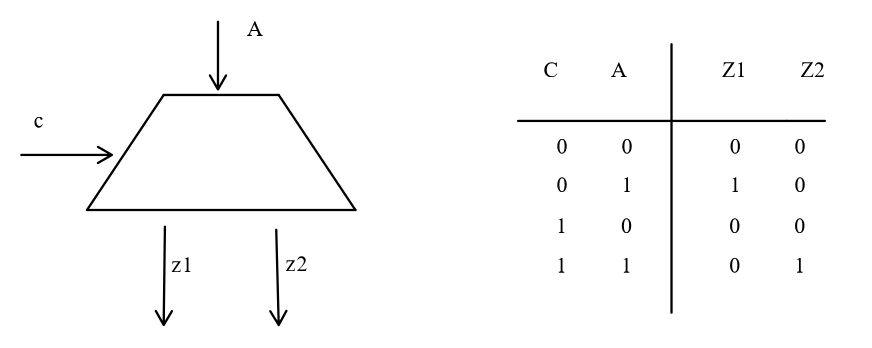
\includegraphics[scale=0.5]{img/demultiplexer1.png}
    \end{figure}
    \vspace*{25px}
    \item \textbf{Espressione Logica}:
    \vspace*{5px}
    \[ z_{1} = \overline{c}a \]
    \[ z_{0} = ca \]
    \vspace*{25px}
    \item \textbf{Rete}:
    \vspace*{5px}
    \begin{figure}[htbp]
    \center
    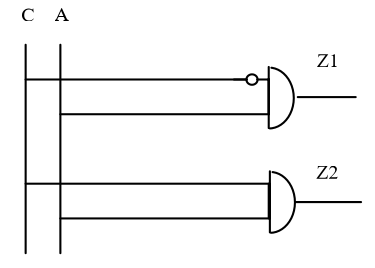
\includegraphics[scale=0.5]{img/demultiplexer2.png}
\end{figure}
\end{enumerate}

\newpage

\subsection{Mappa di Karnaugh}

La Mappa di Karnaugh è un metodo alternativo che permette la produzione di espressioni ottimizzate. Questa è componibile interpretando la tabella di verità. Mostriamo un esempio:

\begin{enumerate}
    \item \textbf{Tabella di Verità}: Assumiamo di essere arrivati a questa fase della logica combinatoria di una funzione arbitraria e di aver ottenuto questa tabella:
    \begin{figure}[htbp]
        \center
        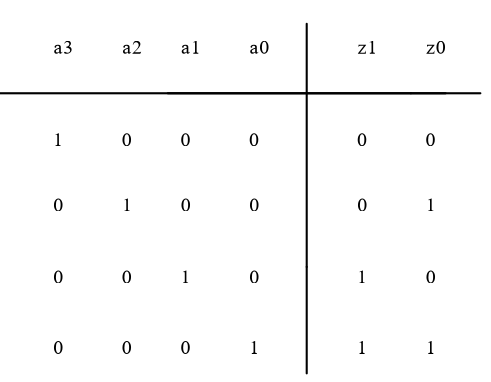
\includegraphics[scale=0.4]{img/tabellaEsempioKarnaugh.png}
    \end{figure}
    \item \textbf{Mappe di Karnaugh}: Ogni colonna in output sarà rappresentata da una singola mappa. Sulle righe avremo le due variabili di input $a_{3},a_{2}$ mentre sulle colonne le restanti variabili di input $a_{1},a_{0}$. 

    
    \begin{figure}[htbp]
        \center
        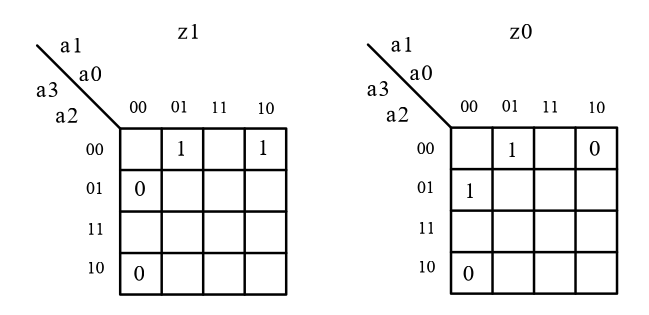
\includegraphics[scale=0.42]{img/tabellaEsempioKarnaugh1.png}
    \end{figure}
    
    Tutte le celle vuote rappresentano valori arbitrari che non variano l'esito nella selezione degli implicanti. Potremmo inserire anche dei trattini $-$

    \item \textbf{Valutazione implicanti ed espressione prodotta}: Bisogna trovare degli \textbf{implicanti}, ossia "blocchi" di $1$ all'interno della mappa in una quantità $2^{k}$. L'esponente $k$ ci permetterà di capire quanti termini stiamo risparmiando rispetto all'espressione originale.

    \begin{figure}[htbp]
        \center
        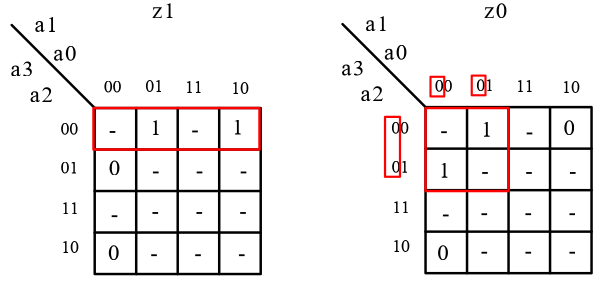
\includegraphics[scale=0.42]{img/tabellaEsempioKarnaugh2.png}
    \end{figure}

    Dunque, l'implicante nella prima mappa si basa sulla riga in cui le prime due variabili sono negate allora $z_{1} = \overline{a_{3}} \: \overline{a_{2}}$, invece nella seconda mappa selezioniamo gli elementi su righe e colonne in comune (cerchiati in rosso), quindi 
    $z_{0} = \overline{a_{3}} \: \overline{a_{1}}$.
    
\end{enumerate}

\newpage

\subsection{Alea}

Generando espressioni ottimizzate con i metodi enunciati
è possibile causare a livello pratico il fenomeno dell'alea.
Dato che ogni colonna di porte genera un tempo di stabilizzazione $\Delta t$ allora è possibile ottenere dei risultati errati per un breve periodo di tempo.
Questo fenomeno è risolvibile aggiungendo un implicante "transitorio" alla mappa che non permetta la sovrapposizione delle operazioni in periodi di tempo non corretti.

\subsection{Full Adder e Sottrazione}

Come possiamo effettuare una sottrazione con i componenti che abbiamo già a disposizione? Basterebbe negare (complemento a due) il secondo termine dell'operazione.

\begin{figure}[htbp]
    \center
    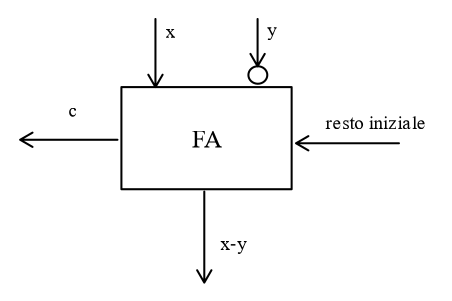
\includegraphics[scale=0.35]{img/fullAdderSott.png}
\end{figure}

\paragraph{Somma o differenza e Full Adder}

La soluzione ottimale è quella di utilizzare un multiplexer al secondo input, stabilendo quindi se negare o meno il termine $y$.

\begin{figure}[htbp]
    \center
    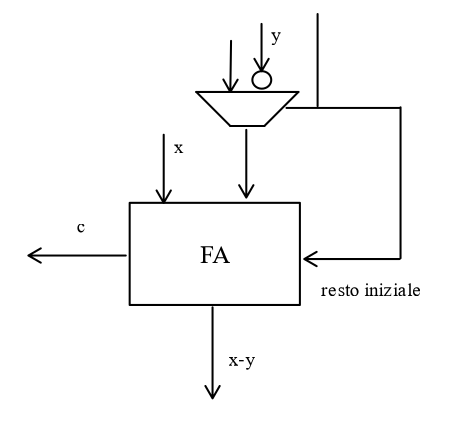
\includegraphics[scale=0.35]{img/fullAdderSott1.png}
\end{figure}

\subsection{Shifter} Mostriamo la rete che ci permette di shiftare a sinistra o a destra i bit in ingresso.

\begin{figure}[htbp]
    \center
    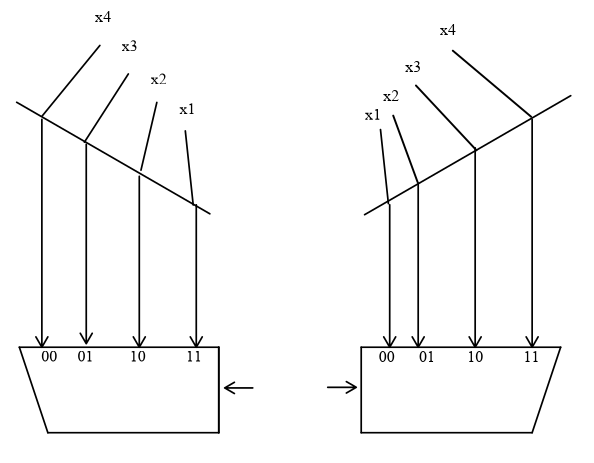
\includegraphics[scale=0.35]{img/shifter_sx_dx.png}
\end{figure}

\newpage

Sceglieremo dunque una posizione di output caratterizzata da quanti zeri di default possiede. Il complemento degli zeri saranno quindi i bit shiftati. Per poter permettere una scelta di direzione (sx, dx) si pone un multiplexer alla colonna successiva dei due shifter, in questo modo si seleziona quale fosse la direzione dello shift effettuato.

\subsection{ALU}

Grazie alla composizione di elementi ricavati dalla gestione di reti basilari e porte logiche possiamo ricavare un nuovo componente, ossia un \textbf{ALU} (Aritmetic Logic Unit). Mostriamo due rappresentazioni:

\begin{figure}[htbp]
    \center
    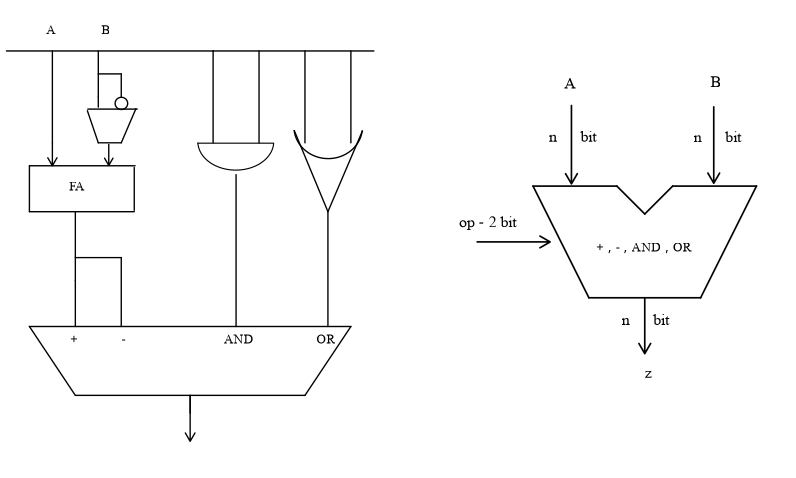
\includegraphics[scale=0.45]{img/ALU1.png}
    %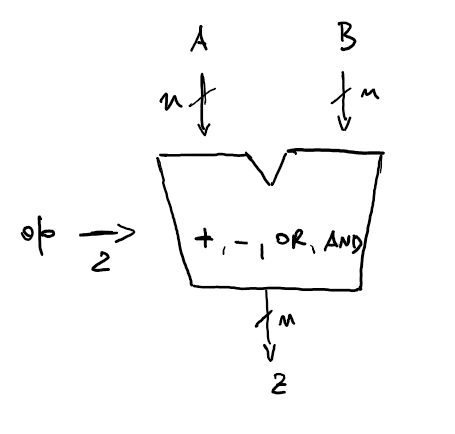
\includegraphics[scale=0.48]{img/ALU2.png}
\end{figure}

Come rappresentato, questa unità ci permette di eseguire operazioni logiche e aritmetica.

\subsection{Arbitro}
L'arbitro è un ulteriore componente che, dato un numero k ingressi, stabilisce quali di questi "vince" in base a se i bit in questione 
    valgono 1 oppure 0. In caso di occorrenza di più bit in ingresso ad uno, vince il primo da sinistra a destra.
\begin{figure}[htbp]
    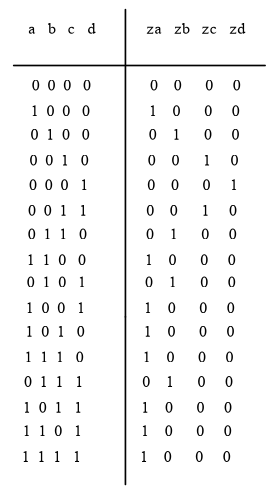
\includegraphics[scale=0.45]{img/tabella_arbitro.png}
    \centering
    \caption{Se osserviamo l'espressione generata osservando gli 1 nelle colonne di output possiamo determinare un upper bound del costo a $2\Delta t$}
\end{figure}

\newpage

\section{Logica Sequenziale}

In questo capitolo si affronta il tipo di logica che tiene conto dei risultati passati grazie ad una memoria. Introduciamo il suo funzionamento di una memoria come rete e successivamente assumeremo ognuno di questi componenti come componenti noti.

Come nella logica combinatoria definiremo quindi delle proprietà/funzioni, ma in questo capitolo queste avranno degli stati, proprio come degli automi.

\vspace*{20px}

\subsection{SR Latch}

Immaginiamo una rete che permette due operazioni, ossia \textbf{set} e \textbf{reset}. Quindi se $w=1$ e $clock=1$ scrive $x$.

\begin{figure}[htbp]
    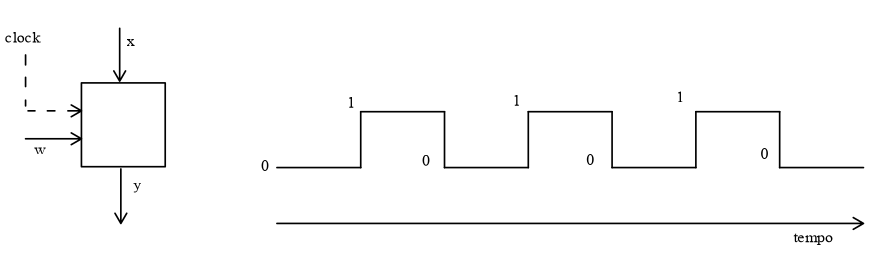
\includegraphics[scale=0.55]{img/memorie1.png}
    \centering
\end{figure}

\vspace*{20px}

\paragraph{Rete Corrispondente}

La rete che ci permette di effettuare queste operazioni è:

\begin{figure}[htbp]
    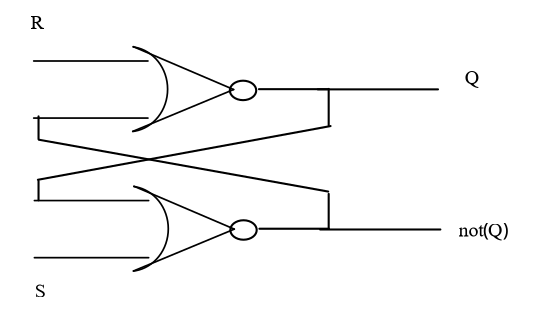
\includegraphics[scale=0.45]{img/memorie2.png}
    \centering
\end{figure}

\begin{enumerate}
    \item \textbf{Set}: $S=1$ il circuito ricorda 1.
    \item \textbf{Reset}: $R=1$ il circuito ricorda 0.
\end{enumerate}

\newpage

\subsection{D Latch} E' necessario imporre che non si possa dare contemporaneamente i valori $S=1, R=1$ nella SR Latch. Dunque possiamo impostare questa condizione con delle porte $AND$ in ingresso:

\begin{figure}[htbp]
    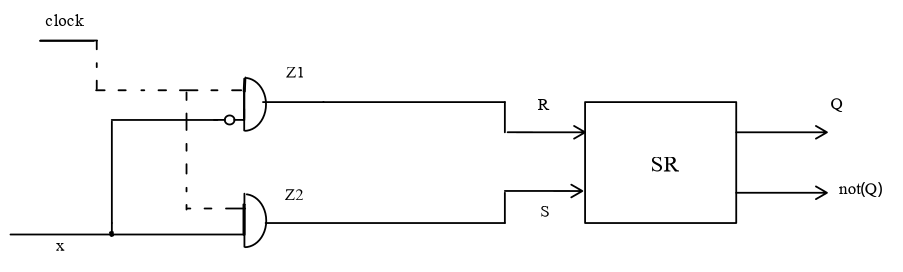
\includegraphics[scale=0.4]{img/memorie3.png}
    \centering
\end{figure}

Abbiamo definito quindi un nuovo componente, ossia il \textbf{D Latch}.

\subsection{D Flip Flop}

Il \textbf{D Flip Flop} si compone di due \textbf{D Latch}:
\begin{enumerate}
    \item \textbf{Master}: Primo D Latch, ha il clock negato in ingresso.
    \item \textbf{Slave}: Primo D Latch, ha il clock affermato in ingresso.
\end{enumerate}

\begin{figure}[htbp]
    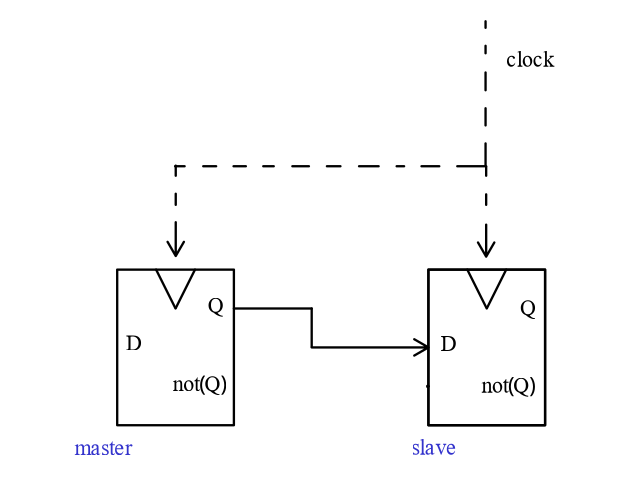
\includegraphics[scale=0.35]{img/D_flip_flop.png}
    \centering
\end{figure}

\begin{figure}[htbp]
    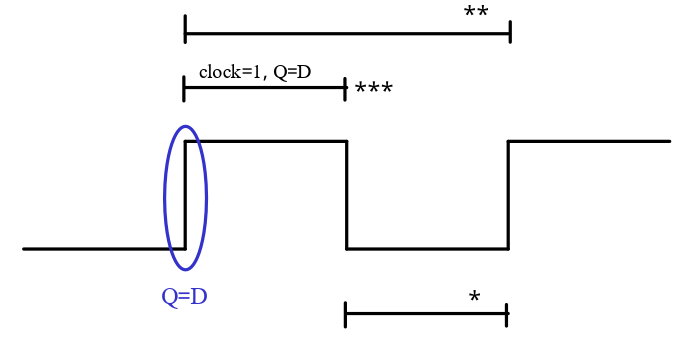
\includegraphics[scale=0.25]{img/clock_flip_flop.png}
    \centering
\end{figure}

\paragraph{Funzionamento} Descriviamo la figura, assumendo che appena prima del periodo (\textbf{**}) è necessario conoscere cosa vogliamo scrivere in input (\textbf{D}).

\begin{enumerate}
    \item \textbf{*}: $clock = 0$, ma lo \textbf{slave} ha già acquisito il valore nella frazione di periodo precedente. Dunque il valore viene mantenuto dato che lo \textbf{slave} ha il clock in ingresso affermato. 
    \item \textbf{**}: Intero periodo in cui verrà mantenuto il valore in ingresso al \textbf{master} poco prima dell'inizio del periodo stesso.
    \item \textbf{***}: Frazione di periodo dove il $clock = 1$, dunque il \textbf{master} ha già portato il suo ingresso \textbf{D} alla sua uscita \textbf{Q}.
\end{enumerate}

\newpage

\subsection{Enabled Flip Flop}

Ponendo un multiplexer all'ingresso del primo \textbf{D Latch} del \textbf{D Flip Flop}
possiamo scegliere di scrivere il nuovo valore in ingresso oppure riscrivere quello corrente. Questo permette allo schema attuale di essere un tipo di memoria \textbf{statica}, essendo che riscriverà il suo valore, indipendentemente da se verrà letta o meno.

\begin{figure}[htbp]
    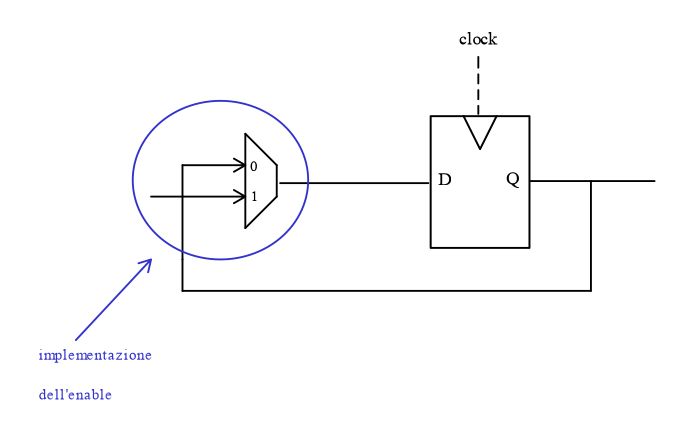
\includegraphics[scale=0.45]{img/enabledFlipFlop.png}
    \centering
\end{figure}

Questo ci permetterà quindi di generare da ora in poi registri da $1$ bit.

\vspace*{20px}

\subsection{Esempio di Sintesi Automa con Memoria}

Vogliamo rappresentare una funzione che ricordi lo stato precedente per poter scegliere tra le possibili scelte.

\vspace*{15px}

\begin{enumerate}
    \item \textbf{Automa e Map Stati}: Assumiamo di voler rappresentare questo automa con una tabella di verità per poterlo convertire in una rete.
    \begin{figure}[htbp]
    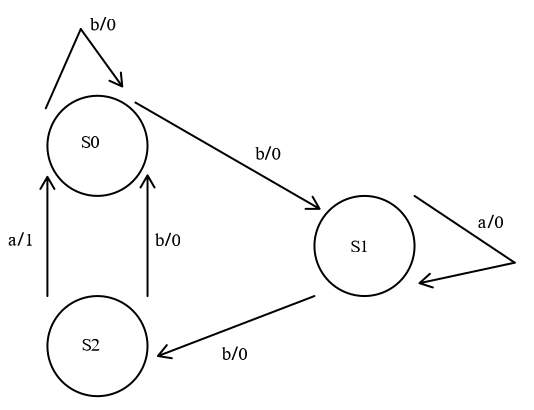
\includegraphics[scale=0.5]{img/automa1.png}
    \centering
\end{figure}

Mappiamo in questo modo gli stati per rappresentarli nella tabella di verità:

    $ S_{0} \mapsto 00 \: \:
    \: \: S_{1} \mapsto 01 \: \:
     S_{2} \mapsto 10 $

    \newpage
        
    \item \textbf{Tabella di Verità}: Rappresentiamo la tabella osservando le possibili scelte 
    
    dell'automa dato.
    \begin{figure}[htbp]
        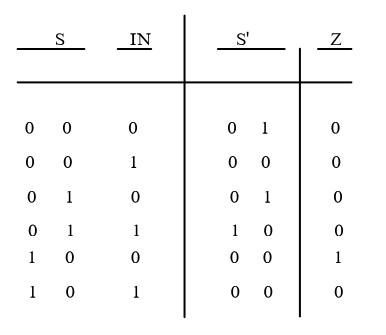
\includegraphics[scale=0.5]{img/TV_automa1.png}
        \centering
    \end{figure}
    
     \item \textbf{Espressione}: Rappresentiamo $3$ espressioni, rispettivamente prima, seconda colonna per gli stati e output.

    \begin{enumerate}
        \item $S_{1}' \: = \: \overline{S_{1}}\:S_{0}\:in $
        \item $S_{0}' \: = \: \overline{S_{1}}\:\overline{S_{0}}\:\overline{in} + \overline{S_{1}}\:S_{0}\:\overline{in} + \overline{S_{1}}\:\overline{in}$
        \item $ z \: = \: S_{1} \: \overline{S_{0}} \: in $
    \end{enumerate}

    \item \textbf{Rete e Componenti}: Rappresentiamo prima i componenti singolarmente, rispettivamente stati di transizione e output, e successivamente mostriamo la complessiva rete generata.

    \begin{figure}[htbp]
        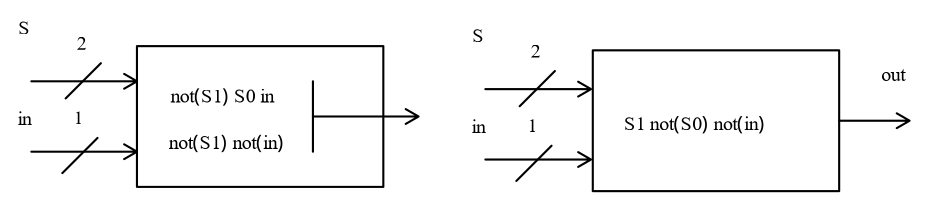
\includegraphics[scale=0.5]{img/rete1_automa1.png}
        \centering
    \end{figure}

    \begin{figure}[htbp]
        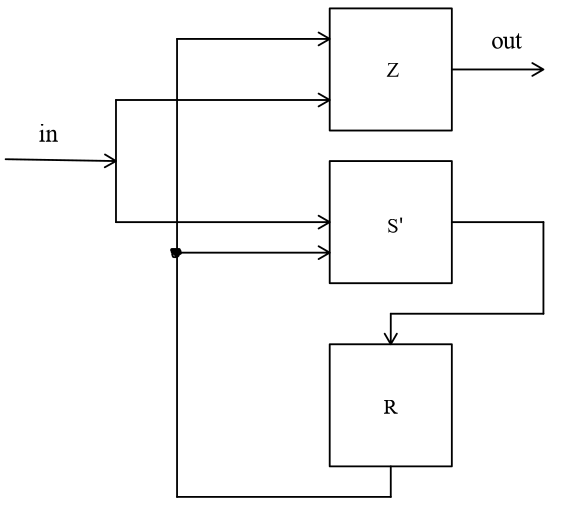
\includegraphics[scale=0.5]{img/rete2_automa1.png}
        \centering
    \end{figure}
    
\end{enumerate}

\newpage

\subsection{Reti di Mealy/Moore}

Grazie all'introduzione dei registri definiti precedentemente, possiamo rappresentare non più solo funzioni ma veri automi a stati finiti.
Prima dei registri era infatti impossibile mantenere le informazioni riguardanti i risultati ottenuti precedentemente. Distinguiamo però due diversi tipi di automi e corrispondenti reti:

\vspace*{20px}

\begin{enumerate}
    \item \textbf{Reti di Mealy}: Reti il cui output dipende sia da \textbf{stato} (informazione mantenuta nei registri), sia da \textbf{input}
    \item \textbf{Reti di Moore}: Reti il cui output dipende esclusivamente dallo stato.
\end{enumerate}

\vspace*{15px}

\begin{figure}[htbp]
    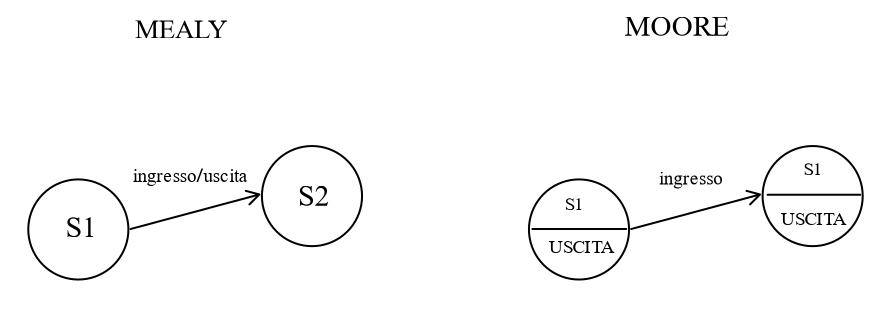
\includegraphics[scale=0.5]{img/mealy_moore.png}
    \centering
\end{figure}

\vspace*{15px}

Parlando quindi di semplici rappresentazioni grafiche, le reti di \textbf{Mealy} hanno input/output sugli archi mentre le reti di \textbf{Moore} hanno solo input, dato che gli output dipendono esclusivamente dallo stato.

\vspace*{20px}

Spesso nelle reti si preferisce utilizzare entrambi gli schemi, sia \textbf{Mealy} sia \textbf{Moore} dato che la seconda tipologia in questione "forza" il passaggio per i registri, evitando in ogni modo la non stabilizzazione della rete.

\vspace*{20px}

Mostriamo un esempio sulle differenze tra \textbf{Mealy} e \textbf{Moore} sull'automa di parità di bit alla successiva pagina.

\newpage

\subsubsection{Automa Parità Bit Mealy/Moore}

Mostiamo l'intera implementazione di un automa che dati $n$ di bit ritorna $1$ se $\# \: di \: 1$ è pari e $0$ se $\# \: di \: 1$ è dispari. 

\begin{enumerate}
    \item \textbf{Versione Mealy}: Seguiamo passo passo la creazione della rete:
    \begin{enumerate}
        \item \textbf{Rappresentazione Automa}: La proprietà descritta sopra sarà così rappresentata in automa:
            \begin{figure}[htbp]
                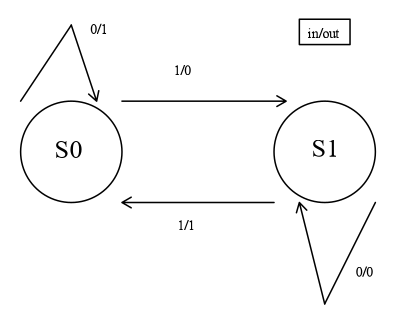
\includegraphics[scale=0.42]{img/parita_mealy.png}
                \centering
            \end{figure}
        \vspace*{10px}
        \item \textbf{Tabella di Verità}: Notiamo che $S_{0} \in \{ 0,1 \}$ e anche $in \in \{ 0,1 \}$
        \begin{figure}[htbp]
            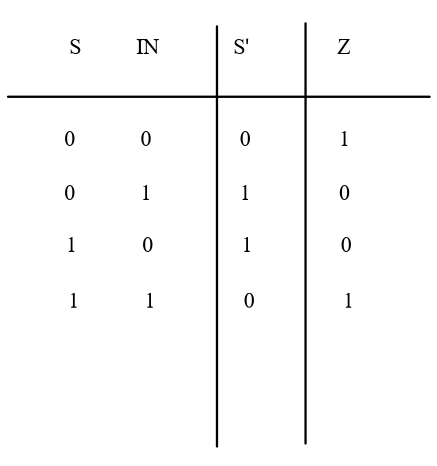
\includegraphics[scale=0.375]{img/tv_paritaMealy.png}
            \centering
        \end{figure}
        \vspace*{-10px}
        \item \textbf{Espressione}: L'espressioni prodotte dall'interpretazione della tabella saranno:
        \[s^{I} = \overline{s}\:in \: + \: s\:\overline{in} \: \: \: \: , \: \: \: \: z = \overline{s}\:\overline{in} \: + \: s\:\overline{in} \]
        \vspace*{-15px}
        \item \textbf{Rete}: Mostriamo la rete prodotta.
        \begin{figure}[htbp]
            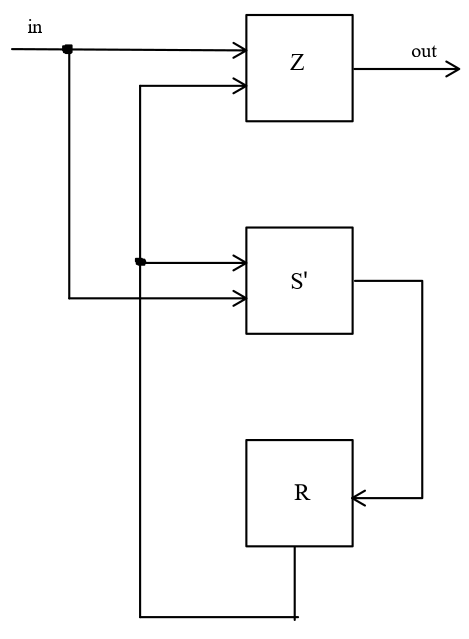
\includegraphics[scale=0.3]{img/parita_mealy_rete.png}
            \centering
        \end{figure}
    \end{enumerate}

\newpage

    \item \textbf{Versione Moore}: Seguiamo il secondo sviluppo notando le differenze:
    \begin{enumerate}
        \item \textbf{Rappresentazione Automa}: Mostriamo la versione \textbf{Moore} dell'automa.
            \begin{figure}[htbp]
                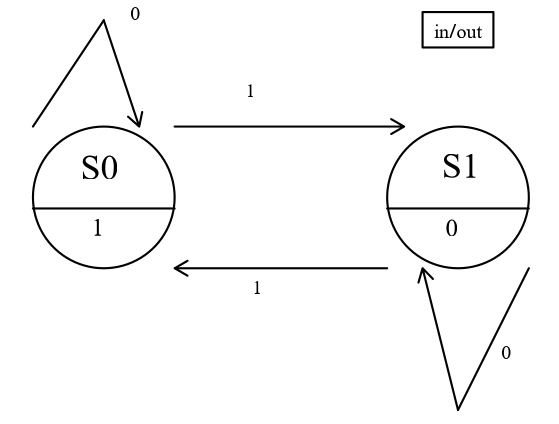
\includegraphics[scale=0.35]{img/paritaMoore.png}
                \centering
            \end{figure}
            \vspace*{10px}
            \item \textbf{Rappresentazione Automa}: Per rappresentare l'automa saranno necessarie due tabelle di verità:
            \begin{figure}[htbp]
                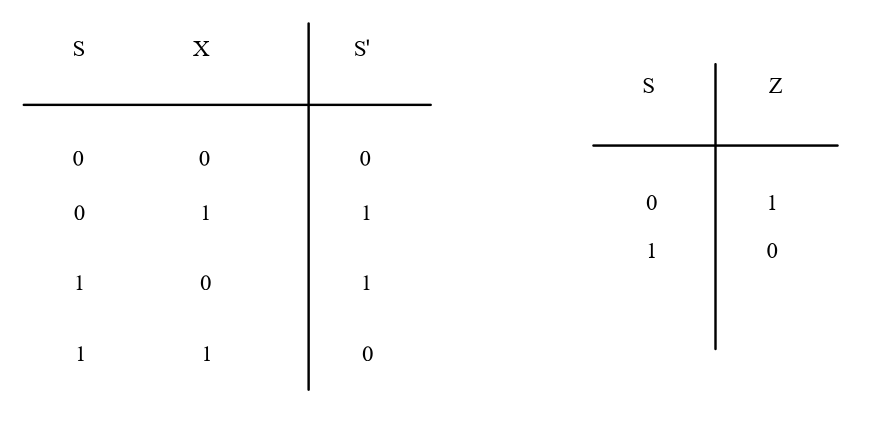
\includegraphics[scale=0.35]{img/paritaMooreTV.png}
                \centering
            \end{figure}
            \vspace*{10px}
            \item \textbf{Espressioni}: Interpretiamo la tabella:
            \[ s^{I} \: = \: \overline{s} \: x \: + s \: \overline{x} \: \: \: \: , \: \: \: \: z \: = \: \overline{s} \]
            \item \textbf{Rete}: Mostriamo la rete prodotta:
            \begin{figure}[htbp]
                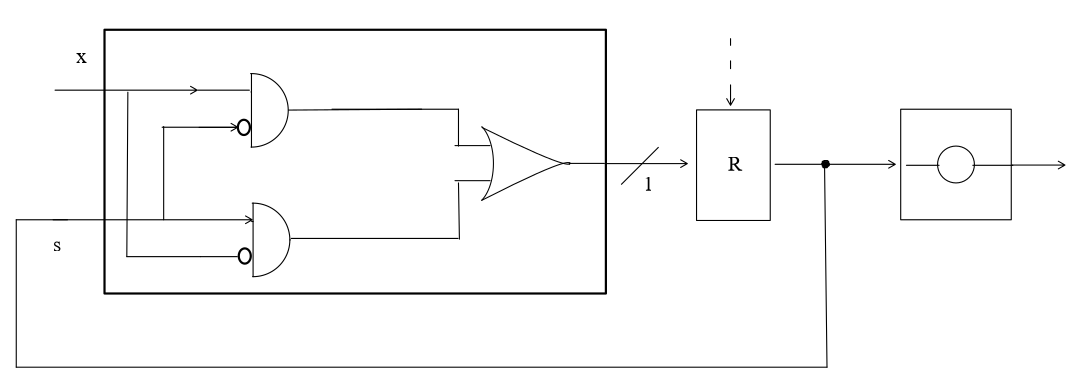
\includegraphics[scale=0.35]{img/paritaMooreRete.png}
                \centering
            \end{figure}
            \item \textbf{Tempi di Stabilizzazione e Clock}: E' necessario che i tempi di stabilizzazione dell'intero circuito siano minori di un ciclo di clock. In questo caso il circuito che produce $s^{I}$ (la prima rete combinatoria) ha un tempo di stabilizzazione di $2 \Delta t$, invece la produzione di $z$ appena dopo il registro si basa solo su una negazione, dunque assumeremo che costi $0 \Delta t$. Dunque elenchiamo tutti i dati in questione:
            \[ r \: = \: max \{ 2 \Delta t \: , \: 0 \Delta t \} \: + \: t_{write} \: \: \: , \: \: \: lunghezzaClock \: \geq \: r \]
    \end{enumerate}
    
\end{enumerate}

\newpage

\subsection{Memorie Statiche/Dinamiche}

Le reti fino ad ora descritte si basavano su dei \textbf{registri} da $1$ bit ciascuno. Questo tipo di memorie hanno particolari caratteristiche. Elenchiamo diversi tipi di memorie:

\subsubsection{Registri - Memorie Statiche}

\begin{enumerate}
    \item $1$ bit di memoria costa circa $20$ \textbf{transistor}.
    \item Effettuano operazioni nell'ordine di tempo dei \textbf{picosecondi} ossia $10^{-12} \:sec$.
    \item Solitamente, si compongono raggruppamenti di questo tipo di memorie massimo da $1024/2048$ bit.
\end{enumerate}

\paragraph{Lettura e Scrittura su Registri}: Possiamo immaginare una memoria come un array di registri da un bit. Sarebbe però necessario, dato un \textbf{indirizzo}, stabilire delle operazioni di \textbf{lettura} e \textbf{scrittura}.

\begin{figure}[htbp]
    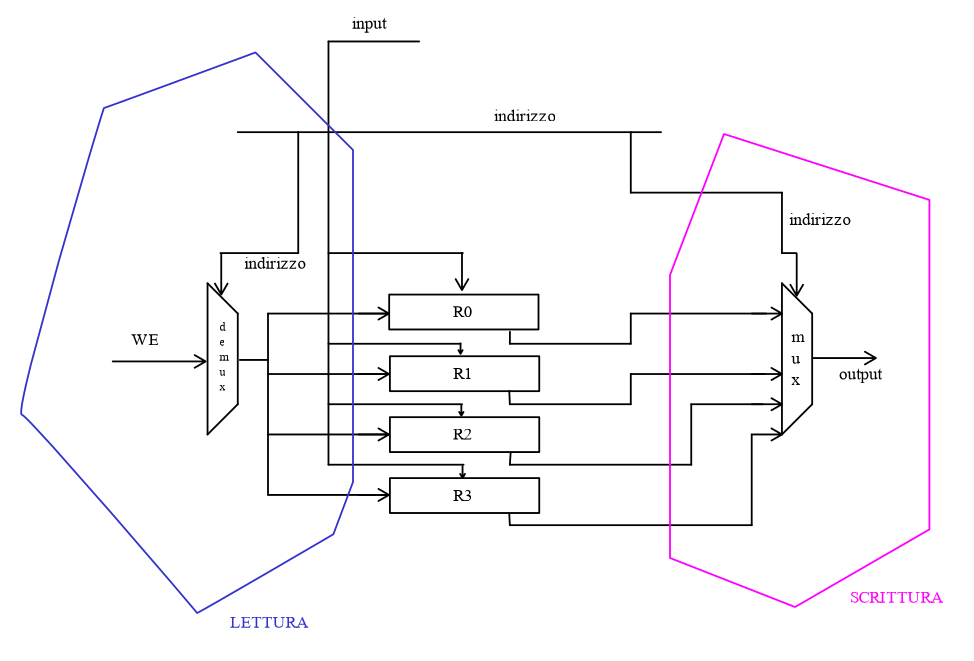
\includegraphics[scale=0.3]{img/letturaScritturaReg.png}
    \centering
\end{figure}

\begin{enumerate}
    \item \textbf{Scrittura}: Possiamo scrivere nei registri in questo modo:
    \begin{enumerate}
        \item Inviamo l'input ad ogni registro (simil broadcast).
        \item Poniamo un \textbf{demultiplexer} con in ingresso il \textbf{write enable (WE)} ed il segnale di controllo sarà l'\textbf{indirizzo}.
    \end{enumerate}
    In questo modo il nuovo input verrà inserito solo nel registro a cui è stato settato il \textbf{write enable} a $1$.
    \item \textbf{Lettura}: La lettura si baserà invece su un concetto leggermente più semplice:
    \begin{enumerate}
        \item Tutte le uscite dei registri entrano in un \textbf{multiplexer}
        \item L'\textbf{indirizzo del registro} di cui vogliamo acquisire il valore sarà utilizzato come \textbf{segnale di controllo} nel multiplexer
    \end{enumerate}
\end{enumerate}

Osservando infine le tabelle di verità richieste per rappresentare lettura e scrittura, verrebbe fuori che la \textbf{scrittura} è più veloce della \textbf{lettura}, dato che la prima richiede $1$ livello di logica e la seconda $2$ livelli di logica. Questo perchè ogni colonna di output della scrittura è "indipendente" dalle altre, non abbiamo un $OR$ tra loro nelle colonne successive, mentre la lettura prende il massimo tra i tempi delle due componenti.

\newpage

\subsubsection{RAM - Memorie Dinamiche} Fino ad ora abbiamo rappresentato memorie che mantenevano nel tempo il loro valore. Le \textbf{memorie dinamiche} invece hanno bisogno di un costante \textbf{refresh} dato che di default non manterranno all'infinito il loro dato, mostriamo il perchè:

\begin{figure}[htbp]
    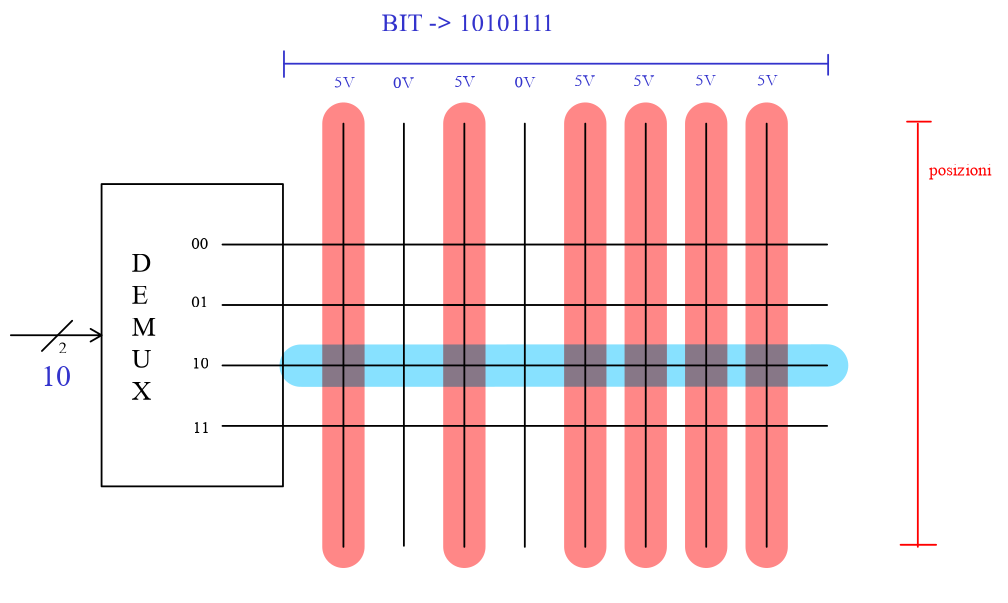
\includegraphics[scale=0.325]{img/memoriaDinamica1.png}
    \centering
\end{figure}

\begin{enumerate}
    \item \textbf{Scrittura}: La scrittura avviene ponendo un voltaggio alto $5v$ sulle colonne e un bit in ingresso rispetto alla posizione sulle righe scelto dal multiplexer. Negli "incroci" di $1$ in riga e colonna viene caricato un condensatore che è posizionato in quella zona.
    (Righe rosse nella rappresentazione).
    \item \textbf{Lettura}: La lettura avviene selezionando la riga che vogliamo leggere, e laddove il condensatore è carico verrà letto $1$, altrimenti $0$ (Riga blu nella rappresentazione).
\end{enumerate}

Vengono definite \textbf{memorie dinamiche} perchè se i condensatori non vengono periodicamente \textbf{refreshate}, queste perderanno la loro carica e quindi il bit che stavano immagazzinando.

\subsection{Classificazione di Memorie}

\begin{enumerate}
    \item \textbf{RAM - Random Access Memory}: Tipologia di memoria caratterizzata dalla possibilità di poter leggere ogni posizione in memoria, come già mostrato in precedenza.
    \item \textbf{ROM - Read Only Memory}: Tipologia di memoria stampata in maniera standard, non permette dunque alcun tipo di scrittura ma solo lettura. Vengono dunque saldati fisicamente i contatti che rappresenteranno $1$ bit di memoria.
    \item \textbf{EPROM - Electrically Programmable Read Only Memory}: Tipologia particolare di \textbf{ROM} che permette di "bruciare" in contatti sulla memoria per poter creare una \textbf{ROM} personalizzata.
    \item \textbf{EEPROM - Erasable Electrically Programmable Read Only Memory}: Simile alla precedente categoria, ma offre la possibilità di effettuare più volte una "bruciatura" dei contatti. Memorie simili vengono utilizzate per i \textbf{BIOS}.

\newpage

    \item \textbf{Memoria Associativa}: Immaginiamo di voler implementare una memoria basata su $<\:chiavi,valori\:>$. E' necessario impostare tutti i livelli necessari in modo tale da poter effettuare un esempio di lettura:
    \begin{enumerate}
        \item \textbf{Livello Comparazione}: Assumendo di avere in memoria delle coppie
        
        $<\:chiave,valore\:>$ allora date delle chiavi abbiamo bisogno di un \textbf{comparatore} che possa stabilire se le chiavi in input siano presenti o meno in memoria.
        \item \textbf{Porta OR}: La porta $OR$ ci permette di stabilire se le chiavi in input sono presenti o meno, ancora prima di cercare il valore corrispondente.
        \item \textbf{Codificatore}: Il codificatore prende in input gli esiti dei comparatori e "interpreta" la posizione dell'$1$, generando un output che verrà utilizzato come segnale di controllo nel multiplexr finale.
        \item \textbf{Multiplexer}: Preso come \textbf{controllo} la posizione dell'$1$, che rappresenta la chiave presente, possiamo utilizzare questo per scegliere grazie al multiplexer il valore in output corrispondente al valore collegato alla chiave iniziale.
    \end{enumerate}

    \item \textbf{Memoria Modulare}: Immaginiamo di avere due zone di memoria ed $n$ bit dedicati agli indirizzi. Determineremo le sottocategorie in base a quale bit utilizziamo per scegliere a quale zona di memoria stiamo facendo riferimento (più/meno significativo).

    \begin{enumerate}
        \item \textbf{Sequenziale}: La Memoria Modulare Sequenziale utilizza il bit più significativo per indicare a quale zona di memoria fa riferimento quell'indirizzo. Questo provoca un utilizzo sequenziale delle celle di memoria disponibili.

    \begin{figure}[htbp]
        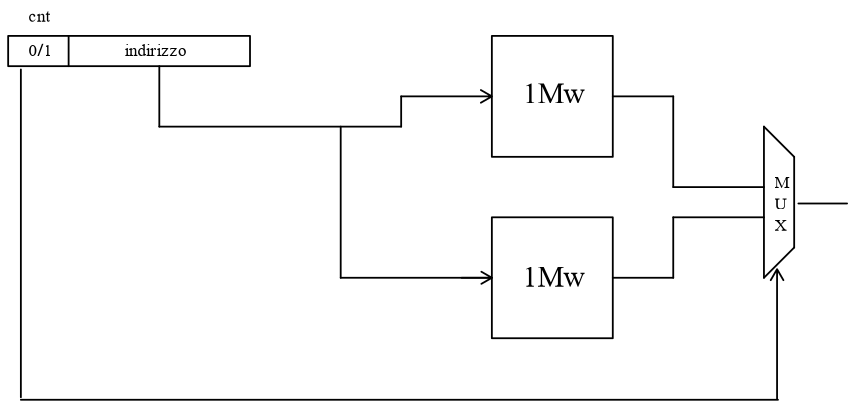
\includegraphics[scale=0.32]{img/memoriaModulare1.png}
        \centering
    \end{figure}
    \vspace*{-5px}
        \item \textbf{Interallacciata}: La Memoria Modulare Interallaciata utilizza il bit meno significativo per indicare a quale zona di memoria fa riferimento quell'indirizzo. Questo provoca un utilizzo alternato tra le due zone delle celle di memoria disponibili.

    \begin{figure}[htbp]
        \includegraphics[scale=0.32]{img/memoriaModulare2.png}
        \centering
    \end{figure}

    \end{enumerate}
        
\end{enumerate}

\newpage

\section{Assembler ARM v7}

In questo capitolo analizzeremo comandi a livello macchina in uno specifico linguaggio

\textit{Assembly} ossia quello dell'architettura \textbf{ARM v7}.

\vspace*{15px}

\subsection{Architettura ARM v7}

Descriviamo gli elementi fondamentali di questo tipo di architettura:

\begin{enumerate}
    \item \textbf{Registri}: I registri sono un tipo di memorie statiche che operano nell'ordine dei picosecondi. In questo tipo specifico di architettura, ogni registro è da $32$ bit. In totale sono presenti 16 registri, che si suddividono in due sottocategorie:
    \begin{enumerate}
        \item \textbf{Registri General Purpose}: Sono registri generici, utilizzati per effettuare operazioni di \textbf{load} e \textbf{store} che permettono l'interazione tra \textbf{memoria} e \textbf{registri}.
        \item \textbf{Registri Speciali}: I registri speciali mantengono valori ricavati da particolari istruzioni oppure contengono informazioni utili al proseguimento dell'esecuzione del programma:
        \begin{enumerate}
            \item \textbf{R15 - PC}: Il \textbf{Program Counter} permette di mantenere l'indirizzo della corrente istruzione. Dunque per andare all'istruzione successiva si effettua:
            \[ PC \: = PC + "1" \]
            \vspace*{-20px}
            \[ PC \: = PC + 4 \]
            \item \textbf{R14 - LR}: Il \textbf{Link Register} mantiene l'indirizzo di ritorno.
            \item \textbf{R13 - SP}: Lo \textbf{Stack Pointer} mantiene l'informazione sullo stack corrente.
            \item \textbf{CPSR}: Il \textbf{Current Program Status Register} contiene varie flag ottenute dalla valutazione di alcuni comandi di comparazione:
            \begin{enumerate}
                \item \textbf {N}: Negative Condition Flag ottenuta da una $CMP$.
                \item \textbf {Z}: Zero Condition Flag ottenuta da una $CMP$.
                \item \textbf {C}: Carry Condition Flag.
                \item \textbf {V}: Overflow Condition Flag.
            \end{enumerate}
        \end{enumerate}
    \end{enumerate}

    \vspace*{15px}
    
    \item \textbf{Memoria}: La memoria possiamo immaginarla come vettore di celle, ognuna da $32$ bit e si suddivide in due grandi categorie:
    \begin{enumerate}
        \item \textbf{Memoria Dati}: Mantiene i dati in memoria.
        \item \textbf{Memoria Istruzioni}: Mantiene le istruzioni da seguire. Ogni \textbf{istruzione} è rappresentata in $32$ bit:
    \end{enumerate}
\end{enumerate}

\newpage

\subsubsection{Descrizione istruzioni da 32 bit}

Ogni istruzione da 32 bit è così composta:

\begin{figure}[htbp]
        \center
        \includegraphics[scale=0.45]{img/istruzione_32bit.png}
    \end{figure}

\begin{enumerate}
    \item \textbf{Condizioni sull'istruzione}: Bit riservati alle condizioni (indicate nelle slide con XX oppure X).
    \item \textbf{Tipo di Operazione}:
    \begin{enumerate}
        \item \textbf{$00$}: Istruzione Operativa
        \item \textbf{$01$}: Istruzione Memoria
        \item \textbf{$00$}: Istruzione di Salto
    \end{enumerate}
    \item \textbf{Registro Destinazione}: Indirizzo del registro in cui scriveremo il risultato 
    
    dell'istruzione corrente.
    \item \textbf{Registro Sorgente 1}: Indirizzo del registro in cui troveremo una sorgente su cui effettuare il calcolo
    \item \textbf{Func, tipo operazione}: Descrive il "titolo" dell'istruzione, dunque a che tipo di istruzione stiamo facendo riferimento.
    \item \textbf{Rappresentazione Costanti}: Questi bit sono dedicati alla rappresentazione di costanti, sono infatti 12 bit che ci permettono di rappresentare, anche grazie agli shift, anche numeri molto grandi.
\end{enumerate}

\paragraph{Rappresentazione Esadecimale} I $32$ bit verranno rappresentati in $8$ cifre esadecimali, ogni cifra rappresenterà "metà" byte di un istruzione.

\begin{figure}[htbp]
        \center
        \includegraphics[scale=0.3]{img/istrMacchina.png}
    \end{figure}

\subsubsection{Opzione THUMB}

Abbiamo stabilito che le istruzioni dell'\textbf{ARM v7} sono rappresentate in $32$ bit. Questa architettura però supporta anche una opzione \textbf{THUMB} (attivabile/disattivabile nella CPSR), che riduce le istruzioni ad una rappresentazione a $16$ bit. Questo può risultare utile su \textbf{microcontrollori} che dispongono di memorie grandi $16/32$ kb. Questo chiaramente ha delle conseguenze, infatti: solo $8$ registri sono considerati utilizzabili, registro dest. e registro $src1$ sono lo stesso, non possiamo utilizzare istr. operative condizionali ecc...

\paragraph{Rappresentazione Esadecimale} Se le istruzioni da $32$ bit necessitavano di $8$ cifre esadecimali, ora le istruzioni in linguaggio macchina saranno rappresentate solo in $4$ cifre.


%\paragraph{Coesistenza} Questa opzione ci permette di far %coesistere operazioni da $32$ e da $16$ bit nello stesso sorgente. 

\newpage

\subsubsection{Descrizione Istruzioni per Categoria (OP, MEM, BRANCH)}

Mostriamo la rappresentazione accurata delle istruzioni in base alla loro tipologia:

\begin{enumerate}
    \item \textbf{Operazionale}: La composizione dei 32 bit in questione è:
    \vspace*{10px}
    \begin{figure}[htbp]
        \center
        \includegraphics[scale=0.22]{img/istrOperazionale.png}
    \end{figure}

    \begin{enumerate}
        \item \textbf{[31:28] bit}: Indica se l'istruzione è o meno condizionale.
        \vspace*{8px}
        \item \textbf{[27:26] bit}: Indica a quale categoria appartiene.
        \vspace*{8px}
        \item \textbf{[25] bit}: Indica se i bit $[11:0]$ rappresenteranno o meno un immediato.
        \vspace*{8px}
        \item \textbf{[24:21] bit}: Indica a quale istruzione stiamo facendo riferimento. (add, sub ...)
        \vspace*{8px}
        \item \textbf{[20] bit}: Indica se l'istruzione setterà o meno le flag, assumendo lo stesso comportamento di una \textbf{cmp}.
        \vspace*{8px}
        \item \textbf{[19:16] bit}: Primo registro sorgente.
        \vspace*{8px}
        \item \textbf{[15:12] bit}: Registro destinazione.
        \vspace*{8px}
        \item \textbf{[11:0] bit}: Sorgente 2, che può essere rappresentata da un registro o da un immediato.
        
        Notiamo nella rappresentazione di \textit{registro-traslato}
        che quando il bit $4$ è settato ad $1$ abbiamo anche la possibilità di shiftare il contenuto del registro dato.
    \end{enumerate}

    \newpage
    
    \item \textbf{Memoria}: La composizione dei 32 bit in questione è:
    
    \begin{figure}[htbp]
        \center
        \includegraphics[scale=0.22]{img/istrMemoria.png}
    \end{figure}

    \begin{enumerate}
        \item \textbf{[31:28] bit}: Indica se l'istruzione è o meno condizionale.
        \vspace*{8px}
        \item \textbf{[27:26] bit}: Indica a quale categoria appartiene.
        \vspace*{8px}
        \item \textbf{[25:20] bit}: Compongono l'effettiva istruzione di \textbf{ldr/str}, in particolare, la \textit{L} ci dice se l'istruzione è di load o store, la \textit{B} invece dice se vogliamo effettuare operazioni grandi $1$ solo byte ecc... Di conseguenza questi $6$ bit compongono la tipologia di istruzione effettiva. 
        \vspace*{8px}
        \item \textbf{[19:16] bit}: Primo registro sorgente.
        \vspace*{8px}
        \item \textbf{[15:12] bit}: Registro destinazione.
        \vspace*{8px}
        \item \textbf{[11:0] bit}: Sorgente 2, che può essere rappresentata da un registro o da un immediato.
    \end{enumerate}

    \item \textbf{Salto}: La composizione dei 32 bit in questione è:
    
    \begin{figure}[htbp]
        \center
        \includegraphics[scale=0.22]{img/istrSalto.png}
    \end{figure}

    \begin{enumerate}
        \item \textbf{[31:28] bit}: Indica se l'istruzione è o meno condizionale.
        \vspace*{8px}
        \item \textbf{[27:26] bit}: Indica a quale categoria appartiene.
        \vspace*{8px}
        \item \textbf{[25:24] bit}: Il primo bit è sempre settato ad $1$, mentre il secondo stabilisce se \textbf{B} oppure \textbf{BL}.
        \vspace*{8px}
        \item \textbf{[23:0] bit}: $24$ bit dedicati all'immediato a verso cui si effettuerà l'operazione di salto (solitamente un etichetta).
    \end{enumerate}
    
\end{enumerate}

\newpage

\subsection{Ciclo del Processore}

Una descritta la memoria ed i registri del processore, è necessario stabilire quali operazioni effettui la \textbf{CPU}. Possiamo dunque assumere che effettui questo:

\begin{lstlisting}[language = JavaScript]
    while (true){
        M[PC] -> istruzione
        decodIstr <- decodifica(istruzione)
        esecuzione(decodIstr)
        scrivi_risultati
        aggiorna(PC)
    }
\end{lstlisting}
\vspace*{-20px}

Dunque, riassumendo, abbiamo a disposizione questi elementi:
\begin{enumerate}
    \item \textbf{CPSR}: Parte dei registri che mantengono le flag su carry, overflow, risultati dei confronti.
    \item \textbf{PC}: Riferimento alla corrente istruzione.
    \item \textbf{REG[16]}: Registri disponibili al processore.
    \item \textbf{MEM$[\:]$}: Memoria dove depositare sorgente e dati.
\end{enumerate}

Da qui in avanti utilizzeremo questi elementi per definire le categorie di istruzioni e la loro semantica.

\paragraph{Semantica ADD} Mostriamo un esempio su un istruzione di $ADD$:

\begin{lstlisting}[language = JavaScript]
    add R0, R1, R2
\end{lstlisting}
\vspace*{-20px}

Questa istruzione somma i contenuti di $R1$ e $R2$ e deposita il risultato in $R0$. Dietro questo si "nasconde" questa semantica:

\begin{lstlisting}[language = JavaScript]
    reg[0] = reg[1] + reg[2]
    PC = PC + 4
\end{lstlisting}
\vspace*{-20px}

Il $+4$ sul \textbf{Program Counter} indica il passaggio all'istruzione successiva, è indicabile anche con $ +"1" $, e vuol dire che stiamo andando avanti di $4$ byte nella lista delle istruzioni, dato che un istruzione è grande esattamente $4$ byte, ossia $32$ bit. Una caratteristica dell'\textbf{Assembly ARM v7} è quella di \textbf{indirizzare al byte}. Questo motiva il $+1$, ossia andare avanti di un unità, ossia 4 byte.

\newpage

\subsection{Tipologie di Istruzioni}

Nell'\textbf{Assembly ARM v7} esiste una classificazioni di istruzioni in base a che genere di operazioni eseguono. Elenchiamole:

\begin{enumerate}
    \item \textbf{Istruzioni Operative}: Questo genere di istruzioni permettono di sommare, sottrarre, dividere o moltiplicare. Mostriamo degli esempi:
\begin{enumerate}
\item \textbf{Somma}: Sommiamo il contenuto in $R2$ e $R3$ depositando il risultato in $R1$.
\begin{lstlisting}[language = JavaScript]
    ADD R1, R2, R3
\end{lstlisting}
\vspace*{-20px}

\item \textbf{Shift Logico a Sx}: Shiftiamo a sinistra (moltiplicazione per 2) il contenuto di $R2$ di $k$ posizioni contenute in $R3$, depositando il risultato in $R1$.
\begin{lstlisting}[language = JavaScript]
    LSL R1, R2, R3
\end{lstlisting}
\vspace*{-20px}

\item \textbf{Shift Aritmetico a Dx}: Shiftiamo a destra (divisione per 2) il contenuto di $R2$ di $k$ posizioni contenute in $R3$, depositando il risultato in $R1$. Questo tipo di shift è detto \textbf{aritmetico} perchè tiene in considerazione del segno del numero sorgente mantenendolo anche dopo lo shift. Dunque pusha $n$ bit ($1$ oppure $0$) stabiliti dal contenuto $R3$ in base a se il numero originale fosse rispettivamente negativo o positivo. 
\begin{lstlisting}[language = JavaScript]
    ASR R1, R2, R3
\end{lstlisting}
\vspace*{-20px}

\item \textbf{Maschera e Cancellazione}: Dato $R1$ sorgente ed $R2$ maschera, questa 

istruzione negherà la maschera data e la porrà in $AND$ con il numero sorgente. Questo causerà un eliminazione dei bit in posizione degli $1$ nella maschera.
\begin{lstlisting}[language = JavaScript]
    BIC R1, R2, R3
\end{lstlisting}
\vspace*{-20px}

A questa classificazione appartengono anche le operazioni logiche come l'$AND$ e l'$OR$.

\end{enumerate}

\item \textbf{Istruzioni Memoria}: Le operazioni principali sono due, ossia rispettivamente caricare nei registri \textbf{(load)} e depositare nella memoria \textbf{(store)}.

\begin{enumerate}
    \item \textbf{Load}:
\begin{lstlisting}[language = JavaScript]
    LDR R1, [indirizzo]
\end{lstlisting}
\vspace*{-20px} 
    \item \textbf{Store}:
\begin{lstlisting}[language = JavaScript]
    STR R1, [indirizzo]
\end{lstlisting}
\vspace*{-20px} 
\end{enumerate}

Notiamo che la prima posizione $R1$ svolge due operazioni diversi tra la \textbf{load} e la \textbf{store}, infatti essendo in entrambi i casi un \textbf{registro}, nel primo caso svolge il ruolo di \textbf{destinazione} dato che stiamo caricando da memoria a registro, mentre nel secondo caso svolge il ruolo di \textbf{sorgente}. Bisogna ora analizzare il secondo parametro, ossia l'\textbf{indirizzo}, che può essere espresso in vari modi in base al tipo di indirizzamento scelto. Elenchiamo a pagina successiva tutte le possibili metodologie.

\newpage

\paragraph{Tipi di indirizzamento} Possiamo indirizzare in vari modi:

\begin{enumerate}
\item \textbf{Indirizzamento Secco}: Mostriamo degli esempi contestualizzati ad uno \textbf{store}:
\begin{lstlisting}[language = JavaScript]
    STR R1, [R2]
\end{lstlisting}
\vspace*{-20px}

Questa metodologia è equivalente a dire $M[R[2]]$. Dunque stiamo prendendo il valore nel registro $R1$ e lo stiamo depositando nella memoria all'indirizzo corrispondente al valore del contenuto di $R2$.

\vspace*{10px}

\item \textbf{Indicizzazione}: Mostriamo degli esempi contestualizzati ad uno \textbf{store}:
\begin{lstlisting}[language = JavaScript]
    STR R1,[R2,R3]
\end{lstlisting}
\vspace*{-20px}

Questa metodologia è equivalente a dire $M[R[2]\: + \:R[3]]$. Dunque stiamo prendendo il valore nel registro $R2$ e lo poniamo come \textbf{base}, mentre $R3$ sarà un \textbf{indice}. In questo modo è possibile effettuare un indicizzazione con somma tra basi ed indici senza ricorrere ad un operazione esplicita di $ADD$. 

Stiamo dunque prendendo il valore nel registro $R1$ e quello in $R2$ e stiamo utilizzando la loro \textbf{somma} per accedere alla \textbf{corrispondente posizione} in \textbf{memoria} per depositare il valore di $R1$. 

\vspace*{10px}

\item \textbf{Post Incremento}: Anche in questo caso mostriamo un operazione di store:
\begin{lstlisting}[language = JavaScript]
    STR R1,[R2],R3
\end{lstlisting}
\vspace*{-20px}

Stiamo quindi:
\begin{enumerate}
    \item Depositando in $M[R2]$ il valore presente in $R1$.
    \item Incrementando il valore di $R2$ con quello di $R3$, in questo modo:
    \[R[2]\: += \: R[3]\]

\end{enumerate}

\vspace*{10px}

\item \textbf{Pre Incremento}: Anche in questo caso mostriamo un operazione di store:
\begin{lstlisting}[language = JavaScript]
    STR R1,[R2,R3]!
\end{lstlisting}
\vspace*{-20px}

Stiamo quindi:
\begin{enumerate}
    \item Incrementando il valore di $R2$ con quello di $R3$, in questo modo:
    \[R[2]\: += \: R[3]\]
    \item Depositando in $M[R2]$ il valore presente in $R1$.
    
\end{enumerate}

\end{enumerate}

\newpage

\item \textbf{Istruzioni Salto}: Le due istruzioni principali di salto sono \textbf{BXX} (branch) e \textbf{BLXX} (branch and link).

\paragraph{Etichette Condizionali delle istruzioni di salto} Queste istruzioni necessitano delle etichette (\textbf{XX} presenti nelle istruzioni sopra elencate), che spesso valutano i valori delle flag presenti nella \textbf{CPSR} ed scelgono se effettuare o meno salti. Elenchiamo le potenziali etichette:

\begin{enumerate}
    \item \textbf{EQ}: Equal, si verifica se la relativa flag nella \textbf{CPSR} sia o meno alzata.
    \item \textbf{GT}: Greater Then, si verifica lo stato delle relativa flag nella \textbf{CPSR}.
    \item \textbf{LT}: Less Then, si verifica lo stato delle relativa flag nella \textbf{CPSR}.
    \item \textbf{NE}: Not Equal, si verifica lo stato della flag \textbf{N} nella \textbf{CPSR}.
\end{enumerate}

Una volta definite le varie etichette (labels), possiamo descrivere i due comandi di salto effettivi:

\begin{enumerate}
    \item \textbf{Branch}: Il branch esegue semplicemente un aggiornamento dell'attuale program counter. Dunque:
    \[ PC = PC \: + \: offset \]
    \item \textbf{Branch and Link}: Il branch and link esegue un aggiornamento dell'attuale program counter, ma salva nel link register la posizione successiva a dove è stato invocato, in modo da poter tornare indietro successivamente, sostituendo ad un ipotetico \textbf{PC} successivo il corrente \textbf{LR}. Dunque:
    \[ PC = PC \: + \: offset \]
    \[ LR = PC \: + \: 4 \]
\end{enumerate}

\end{enumerate}

\paragraph{Istruzioni Etichettate} Mostriamo come sia possibile, anche per altri tipi di istruzioni oltre a quelle di salto, come sia possibile essere etichettate. Mostriamo esempio sulle \textbf{LDM} e \textbf{STM} (load e store multiple).

\begin{enumerate}
    \item \textbf{Possibili Etichette}:
    \begin{enumerate}
        \item \textbf{F}: Full: Partire dall'indirizzo successivo.
        \item \textbf{E}: Empty: Partire dall'indirizzo corrente.
        \item \textbf{A}: Ascending: Sommare 4 al corrente indirizzo.
        \item \textbf{D}: Discending: Sottrarre 4 al corrente indirizzo. 
    \end{enumerate}
    \item \textbf{Esempio}:
\begin{lstlisting}[language = JavaScript]
    STMFD R1!, {R2, R3}
\end{lstlisting}
\vspace*{-20px}

Stiamo discendendo (sottraendo 4) e partendo dal successivo dell'indirizzo dato, ed ogni volta inseriamo il valore dei registri dati nei parametri.

\end{enumerate}

\newpage

\subsection{Schemi di Traduzione: Pseudocodice - ASM ARM}

Elenchiamo e descriviamo schemi noti di codice (if, while, for, ecc...) come traduzione da pseudocodice all'\textbf{ASM ARM V7}.

\begin{enumerate}
    \item \textbf{If Then}: Mostriamo lo schema generico e successivamente un esempio di traduzione.
    \begin{enumerate}
        \item \textbf{Schema Generico}: 
\begin{lstlisting}[language = JavaScript]
        @ test condizione
        BNE not_test
        @ cmd_then
    not_test:
        @ cmd_ext
\end{lstlisting}
        \item \textbf{Pseudocodice}: 
\begin{lstlisting}[language = JavaScript]
    if (x == 7) then x = x + 8
\end{lstlisting}

        \item \textbf{ASM ARM v7}: 
\begin{lstlisting}[language = JavaScript]
        CMP r1, #7
        BNE not_cond
        ADD r1, r1, #8
    not_cond:
        ....
\end{lstlisting}
    \end{enumerate}

    \item \textbf{If Then Else}: In questo caso esistono due schemi di traduzione specchiati, uno che salta nel \textbf{ramo then} e l'altro che salta nel \textbf{ramo else}.
    
    La caratteristica in comune tra i due schemi è quella che bisogna in ogni caso porre una seconda etichetta \textit{oltreThen/oltreElse}. 
    
    Questo perchè eseguendo un else, dovremmo skippare il corpo del then (saltando a \textit{oltreThen}) e lo stesso vale per l'esecuzione di un then (saltando a \textit{oltreElse}).
    Mostriamo lo schema generico e successivamente un esempio di traduzione.

    \vspace*{20px}
    
    \begin{enumerate}
        \item \textbf{Schema Generico}: 
\begin{lstlisting}[language = JavaScript]
        @ test condizione
        BEQ then
        @ corpo else
        B oltrethen //necessario a non eseguire sia else che then
    then:
        @ corpo then
    oltrethen:
        ....
\end{lstlisting}

\newpage

\vspace*{-20px}

        \item \textbf{Pseudocodice}: 
\begin{lstlisting}[language = JavaScript]
    if (x % 2 == 0) then x++
    else x--
\end{lstlisting}

        \item \textbf{ASM ARM v7}: 
\begin{lstlisting}[language = JavaScript]
        ANDS r1,r0,#1 //and e setto FLAG Z
        BNE else
        ADD r0,r0,#1
        B oltre_else
    else:
        SUB r0,r0,#1
    oltre_else:
        ....
\end{lstlisting}
    \end{enumerate}

    \item \textbf{For}: Mostriamo lo schema generico e successivamente un esempio di traduzione. Assumiamo che il corpo del for venga eseguito almeno una volta.
    \begin{enumerate}
        \item \textbf{Schema Generico}: 
\begin{lstlisting}[language = JavaScript]
        @ inizializzazione indice
    loop:
        @ corpo
        @ incremento i
        @ check, se vero loop // BMI loop
\end{lstlisting}
        \item \textbf{Pseudocodice}: 
\begin{lstlisting}[language = JavaScript]
    sum = 0;
    for(i = 1; i<n; i++){
        sum += i;
    }
\end{lstlisting}

        \item \textbf{ASM ARM v7}: 
\begin{lstlisting}[language = JavaScript]
        MOV r0, 1 //variabile sum
        MOV r1, 1 //indice
        //assumiamo che r2 contenga n
    loop:
        ADD r0, r0, r1 //somma
        ADD r1, r1, #1 //incremento indice
        CMP r1, r2 //controllo
        BMI loop
\end{lstlisting}
    \end{enumerate}

Se non fosse possibile assumere che si svolga almeno una iterazione del for basterebbe porre un etichetta aggiuntiva appena fuori il for, per poter effettuare un salto del corpo del ciclo in caso di controllo non superato.

\newpage

    \item \textbf{While}: Mostriamo lo schema generico e successivamente un esempio di traduzione.
    \begin{enumerate}
        \item \textbf{Schema Generico}: 
\begin{lstlisting}[language = JavaScript]
        @ check guardia //se non passa B afterloop
    loop:
        @ corpo
        @ incremento i
        @ check, se vero loop // BMI loop
    afterloop:
        ....
\end{lstlisting}
        \item \textbf{Pseudocodice}: 
\begin{lstlisting}[language = JavaScript]
    while (x > 1) {x = x/2}
\end{lstlisting}

        \item \textbf{ASM ARM v7}: 
\begin{lstlisting}[language = JavaScript]
        MOV r0,#50 //assumiamo x = 50
        CMP r0,#1
        BLT afterloop
    loop:
        LSR r0, r0, #2
        CMP r0, #1
        BGT loop
    afterloop:
        MOV pc,lr
\end{lstlisting}
    \end{enumerate}
    
\end{enumerate}

\subsection{Branch a Contenuto di Registro}

Seguendo uno stile delle istruzioni semplici illustrate fino ad ora, non esiste un vero e proprio comando che ci permetta di saltare al contenuto di un registro invece che ad una semplice etichetta. In realtà esiste un \textbf{BX} che sta per \textit{Branch Exchange Mode}, ma non è coperto dal contenuto di queste dispense.

Utilizzeremo quindi una combinazione di due comandi semplici, ossia:

\begin{lstlisting}[language = JavaScript]
    salto_a_contenuto_reg:
        MOV lr,pc
        MOV pc,Rx
\end{lstlisting}

Questa combinazione ci permetterà di implementare anche funzioni \textbf{higher order}, dato che potremo effettuare un salto ad un indirizzo che abbiamo ad esempio ottenuto come parametro.

\newpage

\section{Microarchitetture}

Questo capitolo si occuperà dell'implementazione effettiva di tutta la logica del capitolo precedente. Dunque sarà necessario fornire delle implementazioni su reti sequenziali di tutte le tipologie di istruzioni mostrate nel capitolo sull'architettura (livello assembler).

\subsection{Tipologie di Parallelismo}

Introduciamo delle tipologie di logica parallela, ossia quel tipo di calcolo che ci permette \textbf{parallelizzare} appunto le operazioni eseguite.

\vspace*{15px}

\begin{enumerate}
    \item \textbf{Parallelismo Spaziale}: Questo tipo di parallelismo si basa sulla divisione di un operazione in tante piccole sotto operazioni indipendenti. Questo ci permetterà di assegnare le piccole operazioni ad \textbf{operatori} diversi. Possiamo rendere chiara l'idea con un esempio pratico. Immaginiamo di voler tradurre un libro di $1000$ pagine. Questo costerà quindi $500$h in termini di tempo. Assumendo che una persona $p_{1}$ possa tradurre $1$ pagina in $30$ minuti, come possiamo parallelizzare il suo lavoro?
    \vspace*{15px}
    \begin{enumerate}
        \item La persona $p_{1}$ può dividere ad esempio il suo lavoro in $10$ parti, dunque $10$ parti da $100$ pagine ciascuna. Assumiamo che questa operazione costi una quantità $K$ in termini di tempo.
        \vspace*{8px}
        \item Assegnando le $10$ parti a $10$ persone diverse, e assumendo che ciascuna persona abbia una velocita di traduzione uguale a quella di $p_{1}$, è possibile notare che in un totale di $50$h si ottiene lo stesso lavoro effettuato da una persona sola in $500$h.
        \vspace*{8px}
        \item Dopo aver stabilito che il tempo impiegato per svolgere il lavoro si calcola con $\frac{T_{seq}}{n} = 50\text{h}$ Bisogna però considerare anche il tempo $K$ impiegato alla prima persona per suddividere il lavoro e quello per ricombinarlo. Dunque il tempo finale\footnote{Chiaramente i due tempi di divisione e ricombinazione non devono essere sostanziali, altrimenti non avrebbe alcun senso effettuare questa strategia di parallelismo.} sarà:
        \[ \frac{T_{seq}}{n} + tempo_{k} + tempo_{ricombina} \]
    \end{enumerate}

    \vspace*{15px}

    \item \textbf{Parallelismo Temporale}: Questo tipo di parallelismo si basa invece su un concetto di \textbf{pipeline}, ossia una sorta di "catena di montaggio". Immaginiamo di avere a disposizione delle stazioni di lavoro. Ciascuna potrebbe avere un tempo di esecuzione diverso dalle altre. 

    Mostriamo e commentiamo degli esempi di pipeline a pagina successiva.

\newpage

    \begin{enumerate}
        \item \textbf{Pipeline a 3 stazioni}: Immaginiamo di avere 3 stazioni di lavoro che elaborano operazioni. Quando un operazione viene elaborata dalla prima stazione viene scaricata nella seconda e così via fino alla completa elaborazione dell'operazione in merito.

        \begin{figure}[htbp]
            \center
            \includegraphics[scale=0.2]{img/Parall_Temporale.png}
        \end{figure}

        \item \textbf{Pipeline combinata al Parallelismo Spaziale}: Immaginiamo di splittare la seconda stazione, in due stazioni diverse, ossia $Str_{21}$ ed $Str_{22}$.

        \begin{figure}[htbp]
            \center
            \includegraphics[scale=0.2]{img/combo_tempo_spazio.png}
        \end{figure}

        Notiamo che in questa versione otteniamo un ottimizzazione dei tempi. Bisogna però categorizzare i tempi citati in questa soluzione.
        
    \end{enumerate}
    
\end{enumerate}

\subsubsection{Costi in Tempo nel Parallelismo}

Analizziamo i costi delle due tipologie di parallelismo:
\begin{enumerate}
    \item \textbf{Costo Parallelismo Spaziale}: Come già stabilito nell'esempio della traduzione del libro:

    \[ \frac{T_{seq}}{n} + tempo_{k} + tempo_{ricombina} \]

\vspace*{8px}
    
    \item \textbf{Costo Parallelismo Temporale}: Definiamo un $t_{i}$ ossia i-esima stazione, ed un $m$ numero di beni da produrre. La formula sarà:
    \[ T \approx (max\{ t_{i} \} * m) + (t_{inizio} + t_{fine})\footnote{Queste quantità saranno trascurabili, essendo il numero di stazioni solitamente molto minore dei beni da produrre.} \]
\end{enumerate}

\newpage

\subsubsection{Latenza e Tempo di Servizio in Parallelismo Temporale}

Stabiliamo le differenze tra queste tipologie di tempo, caratteristiche del Parallelismo Temporale:

\begin{enumerate}
    \item \textbf{Latenza (L)}: Corrisponde alla differenza tra il tempo di fine di un task e il suo tempo d'inizio:
    \[ L = t_{fine} - t_{inizio} \]
    \item \textbf{Tempo di Servizio $T_{s}$}: Corrisponde al tempo che intercorre tra fine di un task e il suo successivo.
    \[ T_{s} = |t_{pred_{i}} \: - \: t_{pred_{i+1}}| \]
\end{enumerate}

\subsection{Esempi di Implementazione Istruzioni Su Processore Single Cycle}

Mostriamo l'implementazione di alcune istruzioni del livello \textbf{assembler} analizzandone i tempi rispetto al ciclo di clock.

\begin{enumerate}
    \item \textbf{Istruzione Operativa}: Mostriamo la rete e descriviamone lo sviluppo temporale:
    
    \begin{figure}[htbp]
        \center
        \includegraphics[scale=0.23]{img/reteOp.png}
    \end{figure}

    \begin{enumerate}
        \item \textbf{Da 0 ad 1}: Tempo di accesso al program counter.
        \item \textbf{Da 1 a 2}: Tempo di accesso alla memoria istruzioni.
        \item \textbf{Da 2 a 3}: Tempo di accesso ai registri e tempo di stabilizzazione dell'estensore (in verde).
        \item \textbf{Da 3 a 4}: Tempo di stabilizzazione dell'ALU.
        \item \textbf{Da 4 a 5}: Tempo di accesso alla memoria dati.
        \item \textbf{Da 5 a 6}: Tempo in cui si fornisce in input al registri l'output della memoria dati.
    \end{enumerate}

\newpage

\item \textbf{Istruzione di Memoria}: Le fasi evidenziate sono simili alla precedente tipologia di operazioni.

    \begin{figure}[htbp]
        \center
        \includegraphics[scale=0.23]{img/reteMem.png}
    \end{figure}

Possiamo però varie differenze sui wire e sulla mancanza di alcune componenti che nelle istruzioni operative risultavano necessarie.

\vspace*{20px}

\item \textbf{Istruzione di Salto}: Mostriamo la rappresentazione: 

    \begin{figure}[htbp]
        \center
        \includegraphics[scale=0.23]{img/reteSalto.png}
    \end{figure}

Notiamo la presenza di alcuni \textbf{multiplexer} necessari per rendere il circuito in grado di processare gli immediati, oppure per poterli shiftare.
    
\end{enumerate}

\newpage

\subsection{Processore Single Cycle}

Immaginiamo un istruzione $ist$ in ASM ed elenchiamo tutte le fasi attraversate dal processore per elaborarla:

\begin{enumerate}
    \item \textbf{Fetch}: Si cerca l'istruzione ASM.
    \item \textbf{Decode}: Decodifica per il processore (ad esempio da istruzione ASM ad esadecimale).
    \item \textbf{Execute}: Elaborazione dell'istruzione in questione.
    \item \textbf{Memory}: Modifiche della memoria apportate dall'elaborazione dell'istruzione (se necessario).
    \item \textbf{Write Back}: Fase che permette la "transizione" all'istruzione successiva.
\end{enumerate}

La caratteristica della \textbf{CPU Single Cycle} è quella di coprire tutte queste fasi in un \textbf{singolo} \textbf{ciclo} di clock. Questo causa cicli di clock molto ampi:

\[ \tau_{SINGLE} \: \approx \: 740 \: \text{picosecondi} \]

    \begin{figure}[htbp]
        \center
        \includegraphics[scale=0.45]{img/implementazione_single_cycle.png}
    \end{figure}

\[ \tau \: \text{(ciclo di clock)} \: = \: \{ 2t_{a}\:+\:t_{ALU}\:+\:2t_{REGISTRI}\:+\:4t_{MUX} \} \]

\vspace*{15px}

Ogni istruzione sarà dunque eseguita in un $\tau$, ma un $\tau$ molto ampio.

\newpage

\subsection{Processore Multi Cycle}

Questo tipo di processore mira a risolvere delle problematiche del processore single cycle, ossia:

\begin{enumerate}
    \item Cicli di clock \textbf{molto ampi}, che coprivano tutti i tipi di operazioni, anche quelle più lente come le LOAD.
    \item Tre circuiti sommatori \textbf{diversi}.
        \item \textbf{Memoria} dati ed istruzioni \textbf{separate}.
\end{enumerate}

Questo tipo di \textbf{CPU} suddivide le operazioni principali in vari \textbf{"stadi"} grazie a dei registri non architetturali che permettono di preservare i dati durante la transizione da uno stadio all'altro. Questo approccio renderà il costo in $\tau$ dipendente dal tipo di operazione effettuata.
La parte di controllo è ancora una rete combinatoria.

\begin{figure}[htbp]
        \center
        \includegraphics[scale=0.45]{img/implementazione_multi_cycle.png}
        \caption{Illustrati in rosso i registri non architetturali, mentre tutti gli altri stadi in colori differenti tra loro}
    \end{figure}

\vspace*{5px}

\[ \tau \: = \: max\{ t_a,\: t_{PC}+t_{MUX}+t_{REGISTRI},\: t_{a},\: t_{MUX}+t_{REGISTRI}  \} \]

\[ \tau_{MULTI} \approx 340 \: \text{picosecondi} \]

\vspace*{20px}

\begin{center}
\begin{tabular}{ |c|c| } %|c|c|c|%
 \hline
  tipo operazione & costo in cicli di clock \\
  \hline
  STR & $4\tau$ \\
  LDR & $5\tau$ \\
  BR & $4\tau$ \\
  OP & $3\tau$ \\
 \hline
\end{tabular}
\end{center}

\newpage

\subsection{Processore Pipeline}

Questo tipo di processore cerca di sfruttare il parallelismo temporale, permettendo alle varie istruzioni di essere elaborate in stadi "paralleli". Mostriamo una rappresentazione dello schema logico di pipeline:

\begin{figure}[htbp]
        \center
        \includegraphics[scale=0.6]{img/pipeline_senza_dip.png}
    \end{figure}

Questa tipologia di schema permette, una volta raggiunta un esecuzione \textbf{a regime}, di elaborare un istruzione in $1\overline{\tau}$ ciascuna, indipendentemente dal tipo. Ovviamente $\overline{\tau} << \tau$, quindi il ciclo di clock della CPU \textbf{pipeline} è molto meno ampio di quella in \textbf{single cycle}.

    \begin{figure}[htbp]
        \center
        \includegraphics[scale=0.375]{img/implementazione_pipeline.png}
    \end{figure}

Notiamo che nel processore a pipeline la zona di controllo è una \textbf{rete sequenziale}. E' infatti necessario che anche la zona di controllo possa mantenere informazioni tra i vari stadi grazie a dei registri non architetturali.

\vspace*{15px}

Ricordiamo che ogni istruzione causa un cambio di stato alla memoria complessiva. Di conseguenza due istruzioni potrebbero essere \textbf{dipendenti} tra loro in questo schema. Vanno dunque gestite queste situazioni.

\newpage

\subsubsection{Dipendenze Logiche - Condizioni di Bernstein}

Stabiliamo le dipendenze tra istruzioni consecutive grazie alle \textbf{Condizioni} di \textbf{Bernstein}:

\[ \text{Se} \:\:\: R_{1} \: \cap \: W_{2} \:  = \: \emptyset \:\:\: , \:\:\: R_{2} \: \cap \: W_{1} = \: \emptyset \:\:\: , \:\:\: W_{1} \: \cap \: W_{2} = \: \emptyset \]

\vspace*{-10px}

\[ \text{allora}  \:\:\: OP_{1};OP_{2} \: \equiv \: OP_{2};OP_{1} \]

Ossia, possiamo invertire l'ordine di due istruzioni generiche se queste non spezzano le Condizioni di Bernstein.

Esistono due modi per risolvere queste tipologie di dipendenze:

\vspace*{20px}

\begin{enumerate}
    \item \textbf{Forwarding}: Una delle soluzioni è fornire alla seconda istruzione in elaborazione i risultati della prima istruzione con la quale è presente dipendenza logica. Si tenta dunque di \textbf{inoltrare} i \textbf{risultati} della \textbf{prima istruzione} (disponibili nello stadio Memory o Write Back) \textbf{verso} la \textbf{seconda istruzione} dipendente (attualmente posizionata nello stadio Execute).
    \begin{figure}[htbp]
        \center
        \includegraphics[scale=0.375]{img/forwarding.png}
    \end{figure}


    Questa soluzione ha delle limitazioni, infatti se un ipotetica seconda istruzione dovesse dipendere da una prima istruzione LDR (che impiega più tempo per scrivere i risultati) questa tecnica non risulterebbe sufficiente.

    \vspace*{10px}

    \item \textbf{Creazione Stalli}: In situazioni come quella appena descritta l'unico modo per risolvere la dipendenza logica è la creazione di tempi vuoti (\textbf{stalli}) che permettano la scrittura dei risultati necessari allo svolgimento della seconda operazione.
\end{enumerate}

\newpage

\subsubsection{Dipendenze sul Controllo}

Anche le \textbf{istruzioni} di \textbf{salto} creano problemi alla pipeline, dato che si starebbero elaborando \textbf{istruzioni da ignorare} successivamente.

\begin{figure}[htbp]
    \center
    \includegraphics[scale=0.45]{img/forwarding_controllo.png}
\end{figure}

Le dipendenze di controllo si verificano quando la decisione di quale sia la prossima istruzione da prelevare non sia ancora
stata presa al momento del fetch; possono essere gestite prevedendo quale sia l’istruzione da leggere e svuotando la pipeline se la previsione si rivela errata,
o mettendo in stallo la pipeline finché la decisione se saltare o meno non sia stata presa.

\[ \boxed{\text{Tempi senza Dipendenze:} \;\;\; m\tau \: + \: 4\tau} \]


\[ \boxed{\text{Tempi con Dipendenze:} \;\;\; m\tau \: + \: (\#stalli\_dip\_logiche)\tau \: + \: (\#salti\_presi)2\tau} \]


In realtà tutti i segnali di controllo inviati ai \textbf{MUX} per regolare l'utilizzo dei forwarding vengono gestiti dall'\textbf{hazard unit}. 

\newpage

\end{document}